\documentclass[11pt,a4paper]{report}

% ==============================================================================
% PACKAGES ET CONFIGURATION TYPOGRAPHIQUE
% ==============================================================================
\usepackage[utf8]{inputenc}
\usepackage[T1]{fontenc}
\usepackage[french]{babel}
\usepackage{lmodern}
\usepackage{amsmath,amssymb,amsfonts,amsthm}
\usepackage{graphicx}
\usepackage{xcolor}
\usepackage{geometry}
\usepackage{fancyhdr}
\usepackage{booktabs}
\usepackage{tabularx}
\usepackage{array}
\usepackage{listings}
\usepackage{tcolorbox}
\usepackage{tikz}
\usetikzlibrary{shapes.geometric,arrows.meta,positioning,calc,fit}
\usepackage[colorlinks=true,linkcolor=navyblue,citecolor=navyblue,urlcolor=navyblue]{hyperref}

\geometry{top=2.5cm, bottom=2.5cm, left=2.3cm, right=2.3cm, headheight=14pt}

% --- Palette ---
\definecolor{navyblue}{RGB}{26, 54, 93}
\definecolor{royalblue}{RGB}{43, 108, 176}
\definecolor{darkcharcoal}{RGB}{45, 55, 72}
\definecolor{lightbg}{RGB}{247, 250, 252}
\definecolor{accentred}{RGB}{155, 44, 44}
\definecolor{tealhpc}{RGB}{44, 122, 123}
\definecolor{goldline}{RGB}{214, 158, 46}

% --- Boîtes ---
\tcbuselibrary{skins,breakable}
\newtcolorbox{cadreconcept}[1][]{
    colback=lightbg, colframe=navyblue, fonttitle=\bfseries\color{white},
    colbacktitle=navyblue, enhanced,
    attach boxed title to top left={yshift=-2mm, xshift=5mm},
    boxed title style={sharp corners, boxrule=0pt},
    boxrule=0.8pt, arc=3pt, title=#1, breakable
}
\newtcolorbox{encadreresume}[1][]{
    colback=tealhpc!5!white, colframe=tealhpc, fonttitle=\bfseries\color{white},
    colbacktitle=tealhpc, enhanced,
    attach boxed title to top left={yshift=-2mm, xshift=5mm},
    boxed title style={sharp corners, boxrule=0pt},
    boxrule=0.8pt, arc=3pt, title=#1, breakable
}
\newtcolorbox{encadreattention}[1][]{
    colback=yellow!5!white, colframe=goldline, fonttitle=\bfseries\color{navyblue},
    colbacktitle=goldline!30!white, enhanced, boxrule=0.8pt, arc=2pt,
    title=#1, breakable
}

% --- Listings ---
\lstset{
    language=Python,
    basicstyle=\ttfamily\footnotesize\color{darkcharcoal},
    keywordstyle=\bfseries\color{royalblue},
    stringstyle=\color{accentred},
    commentstyle=\itshape\color{gray},
    numbers=left, numberstyle=\tiny\color{gray}, stepnumber=1, numbersep=8pt,
    backgroundcolor=\color{lightbg},
    showspaces=false, showstringspaces=false, showtabs=false,
    frame=single, rulecolor=\color{gray!30}, tabsize=4, captionpos=b,
    breaklines=true, breakatwhitespace=false,
    xleftmargin=15pt, framexleftmargin=15pt,
    inputencoding=utf8, extendedchars=true,
    literate=
        {é}{{\'e}}1 {è}{{\`e}}1 {à}{{\`a}}1 {ê}{{\^e}}1 {ë}{{\"e}}1
        {î}{{\^i}}1 {ï}{{\"i}}1 {ô}{{\^o}}1 {û}{{\^u}}1 {ù}{{\`u}}1
        {ç}{{\c{c}}}1 {É}{{\'E}}1 {È}{{\`E}}1 {À}{{\`A}}1 {œ}{{\oe}}1
        {µ}{{$\mu$}}1 {°}{{$^\circ$}}1 {—}{{---}}1 {’}{{'}}1 {…}{{\dots}}1
}

% --- Théorèmes ---
\theoremstyle{plain}
\newtheorem{theorem}{Théorème}[chapter]
\newtheorem{proposition}{Proposition}[chapter]
\newtheorem{lemma}{Lemme}[chapter]
\theoremstyle{definition}
\newtheorem{definition}{Définition}[chapter]
\theoremstyle{remark}
\newtheorem{remark}{Remarque}[chapter]

\newcommand{\Rzero}{\mathcal{R}_0}

% --- En-têtes et pieds de page ---
\pagestyle{fancy}
\fancyhf{}
\fancyhead[L]{\small\itshape Implémentation du modèle d'infection par le VIH-SIDA -- BLAS, LAPACK et Intel MKL}
\fancyhead[R]{\small\bfseries\color{navyblue} Groupe 5}
\fancyfoot[L]{\small\color{gray} ENSGMM1 -- UNSTIM (Abomey)\quad|\quad UE : Outils de calcul scientifique\quad|\quad Groupe 5}
\fancyfoot[R]{\small\bfseries\color{navyblue} Page \thepage}
\renewcommand{\headrulewidth}{0.5pt}
\renewcommand{\footrulewidth}{0.5pt}
\renewcommand{\footrule}{\color{goldline}\hrule width\headwidth height\footrulewidth\vskip-\footrulewidth}

\fancypagestyle{plain}{
    \fancyhf{}
    \fancyfoot[L]{\small\color{gray} ENSGMM1 -- UNSTIM (Abomey)\quad|\quad UE : Outils de calcul scientifique\quad|\quad Groupe 5}
    \fancyfoot[R]{\small\bfseries\color{navyblue} Page \thepage}
    \renewcommand{\headrulewidth}{0pt}
    \renewcommand{\footrulewidth}{0.5pt}
}

\begin{document}

% ==============================================================================
% PAGE DE GARDE
% ==============================================================================
\begin{titlepage}
    \begin{tikzpicture}[remember picture, overlay]
        \draw[line width=1.5pt, color=navyblue]
            ($(current page.north west) + (1.2cm,-1.2cm)$) rectangle
            ($(current page.south east) + (-1.2cm,1.2cm)$);
        \draw[line width=0.6pt, color=goldline]
            ($(current page.north west) + (1.35cm,-1.35cm)$) rectangle
            ($(current page.south east) + (-1.35cm,1.35cm)$);
    \end{tikzpicture}

    \centering
    \vspace*{-0.9cm}
    \noindent
    \begin{minipage}[t]{0.40\textwidth}
        \raggedright
        \hspace*{0.3cm}
\includegraphics[height=2.5cm]{figures/logo_unstim.png}
    \end{minipage}%
    \hfill
    \begin{minipage}[t]{0.40\textwidth}
        \raggedleft
        
\includegraphics[height=2.5cm]{figures/logo_ensgmm.png}\hspace*{0.3cm}
    \end{minipage}

    \vspace{0.4cm}

    {\fontsize{11}{14}\selectfont \textsc{\textbf{République du Bénin}}}\\[0.15cm]
    {\fontsize{10}{13}\selectfont \textbf{Ministère de l'Enseignement Supérieur et de la Recherche Scientifique}}\\[0.25cm]
    {\fontsize{12}{15}\selectfont \textsc{\textbf{Université Nationale des Sciences, Technologies,}}}\\[0.1cm]
    {\fontsize{12}{15}\selectfont \textsc{\textbf{Ingénierie et Mathématiques d'Abomey (UNSTIM)}}}\\[0.3cm]
    {\fontsize{13}{16}\selectfont \textcolor{navyblue}{\textbf{École Nationale Supérieure de Génie Mathématique et Modélisation (ENSGMM)}}}

    \vspace{0.4cm}
    \textcolor{goldline}{\rule{0.8\textwidth}{1.2pt}}
    \vspace{0.5cm}

    \begin{tcolorbox}[colback=navyblue!5!white, colframe=navyblue, arc=4pt,
        boxrule=1.2pt, width=0.95\textwidth, halign=center]
        \vspace{0.3cm}
        {\fontsize{20}{24}\selectfont \textbf{\textcolor{navyblue}{Implémentation du modèle d'infection}}}\\[0.2cm]
        {\fontsize{22}{26}\selectfont \textbf{\textcolor{accentred}{par le VIH-SIDA}}}\\[0.35cm]
        {\fontsize{11}{14}\selectfont \textbf{\textit{Modèles intra-hôte et de population : analyse mathématique,}}}\\[0.1cm]
        {\fontsize{11}{14}\selectfont \textbf{\textit{stabilité et résolution numérique avec}}}\\[0.1cm]
        {\fontsize{11}{14}\selectfont \textbf{\textit{BLAS, LAPACK et Intel MKL en Python}}}
        \vspace{0.3cm}
    \end{tcolorbox}

    \vspace{0.6cm}

    {\fontsize{13}{16}\selectfont \textbf{\textcolor{navyblue}{\underline{Équipe de projet -- Groupe 5}}}}\\[0.35cm]
    {\large \textbf{ADOGOUN}} Déo Gracias Mahugnon\\[0.15cm]
    {\large \textbf{BIAHOU}} Ahossou Junior Marie-Clémenceau\\[0.15cm]
    {\large \textbf{SYLLA IMOROU}} Izou Dine

    \vfill

    \begin{tcolorbox}[colback=lightbg, colframe=gray!40, boxrule=0.5pt, arc=2pt, width=0.92\textwidth]
        \centering
        \small
        \textbf{Promotion :} ENSGMM1 \quad $\bullet$ \quad \textbf{UE :} Outils de calcul scientifique\\[0.1cm]
        \textbf{Année académique :} 2026--2027\\[0.15cm]
        \textbf{Sous la direction de :} \textbf{\textcolor{navyblue}{Dr. Carlos AGOSSOU}}
    \end{tcolorbox}
    \vspace*{-0.2cm}
\end{titlepage}

% ==============================================================================
% TABLE DES MATIÈRES
% ==============================================================================
\newpage
\pagenumbering{arabic}   % la numérotation commence à 1 à la table des matières
\tableofcontents
\newpage

% ==============================================================================
% INTRODUCTION
% ==============================================================================
\chapter*{Introduction}
\addcontentsline{toc}{chapter}{Introduction}

\begin{cadreconcept}[Résumé en clair : de quoi parle ce projet ?]
Ce travail étudie la dynamique du virus de l'immunodéficience humaine (VIH) à deux échelles complémentaires :
\begin{enumerate}
    \item \textbf{À l'échelle du patient (modèle intra-hôte) :} comment le virus infecte les lymphocytes T CD4+ du sang et comment un traitement antirétroviral bloque cette infection ;
    \item \textbf{À l'échelle de la population (modèle épidémiologique) :} comment l'épidémie se propage entre personnes saines, personnes infectées sans symptômes et personnes au stade SIDA.
\end{enumerate}
Pour résoudre ces équations de façon fiable et rapide, nous nous appuyons sur la pile logicielle standard du calcul scientifique : \textbf{Intel MKL}, qui fournit des implémentations optimisées de \textbf{BLAS} et de \textbf{LAPACK}, appelées depuis \textbf{Python}.
\end{cadreconcept}

\vspace{0.3cm}
\noindent\textbf{Pourquoi un tel sujet ?}
Un modèle de dynamique virale est un système d'équations différentielles non linéaires \emph{raide} : certaines grandeurs évoluent en minutes (le virus libre), d'autres en mois (les lymphocytes). Sa résolution fiable demande des solveurs d'algèbre linéaire robustes (factorisation LU, valeurs propres, conditionnement) : c'est exactement le rôle de LAPACK, lui-même construit sur les opérations de base de BLAS.

\vspace{0.3cm}
\noindent\textbf{Les quatre objectifs du travail :}
\begin{enumerate}
    \item Comprendre l'articulation de la pile logicielle \textbf{MKL / BLAS / LAPACK} et savoir la configurer et l'appeler depuis Python ;
    \item Formuler et analyser mathématiquement le modèle intra-hôte (positivité, bornitude, nombre de reproduction $\Rzero$, stabilité) et le modèle de population $S,I_1,I_2$ ;
    \item Résoudre numériquement ces modèles avec des routines LAPACK (\texttt{DGESV}, \texttt{DGEEQU}, \texttt{DGEEV}), en maîtrisant la raideur grâce à un schéma d'Euler implicite, puis en interpréter les résultats sur le plan médical ;
    \item Mesurer le gain de performance apporté par BLAS/LAPACK par rapport à un code Python naïf.
\end{enumerate}

\vspace{0.3cm}
\noindent\textbf{Organisation du rapport.}
Les chapitres~1 à~4 présentent les outils (MKL, BLAS, LAPACK, installation). Le chapitre~5 rappelle le contexte biologique. Les chapitres~6 à~9 traitent du modèle intra-hôte (analyse, méthodes numériques, intégration, résultats). Le chapitre~10 est consacré au modèle de population et le chapitre~11 au benchmark de performance. Le code complet figure en annexe.

% ==============================================================================
% CHAPITRE 1 : INTEL MKL
% ==============================================================================
\chapter{Présentation d'Intel MKL (oneMKL)}

\section{Qu'est-ce qu'Intel MKL ?}

\begin{cadreconcept}[Définition]
\textbf{Intel MKL} (\textit{Math Kernel Library}, aujourd'hui intégrée à la suite \textbf{Intel oneAPI} sous le nom \textbf{oneMKL}) est une bibliothèque de calcul numérique hautement optimisée pour les processeurs Intel. Elle fournit, entre autres, des implémentations de \textbf{BLAS} et de \textbf{LAPACK}.
\end{cadreconcept}

Il faut bien distinguer trois notions qui sont souvent confondues :
\begin{itemize}
    \item \textbf{BLAS} est une \emph{spécification} : une liste standardisée d'opérations élémentaires d'algèbre linéaire (chapitre~2) ;
    \item \textbf{LAPACK} est une \emph{bibliothèque algorithmique} qui résout de vrais problèmes (systèmes linéaires, valeurs propres, \dots) en s'appuyant sur BLAS (chapitre~3) ;
    \item \textbf{Intel MKL} est une \emph{implémentation industrielle optimisée} de ces deux interfaces, avec des noyaux de calcul adaptés au matériel.
\end{itemize}
Un programme écrit une seule fois contre l'interface standard (par exemple l'appel à \texttt{DGEMM}) peut ainsi être exécuté avec différentes implémentations, sans modification du code source.

\section{Domaines couverts}

Au-delà de BLAS et de LAPACK, oneMKL regroupe plusieurs familles de routines (tableau~\ref{tab:mkl_domaines}).

\begin{table}[ht]
\centering
\caption{Principaux domaines couverts par Intel oneMKL.}
\label{tab:mkl_domaines}
\begin{tabularx}{\textwidth}{l X}
\toprule
\textbf{Domaine} & \textbf{Contenu} \\
\midrule
BLAS et LAPACK & Algèbre linéaire dense : produits matriciels, factorisations LU/QR/Cholesky, valeurs propres, SVD. \\
Algèbre linéaire creuse & BLAS creux, solveurs directs (PARDISO) et itératifs. \\
Transformées de Fourier & FFT mono- et multidimensionnelles. \\
Fonctions vectorielles & Fonctions mathématiques appliquées à des vecteurs entiers (exponentielle, logarithme, \dots). \\
Statistiques et aléatoire & Générateurs de nombres aléatoires, statistiques de base. \\
\bottomrule
\end{tabularx}
\end{table}

Dans ce projet, seuls BLAS et LAPACK sont utilisés : les produits matriciels (\texttt{DGEMM}), la résolution de systèmes (\texttt{DGESV}), l'équilibrage (\texttt{DGEEQU}), l'estimation du conditionnement (\texttt{DGECON}) et le calcul spectral (\texttt{DGEEV}).

\section{Avantages et alternatives du marché}

Les performances d'oneMKL reposent sur trois leviers matériels :
\begin{enumerate}
    \item \textbf{La vectorisation SIMD} (AVX2, AVX-512) : une seule instruction traite plusieurs nombres flottants à la fois ;
    \item \textbf{Le parallélisme multi-cœurs} (threads OpenMP) : les grandes matrices sont découpées en blocs répartis sur les cœurs ;
    \item \textbf{Le choix dynamique du noyau} : au lancement, la bibliothèque détecte le modèle de processeur et sélectionne la version du code la mieux adaptée.
\end{enumerate}

Le tableau~\ref{tab:alternatives_mkl} compare les principales implémentations disponibles.

\begin{table}[ht]
\centering
\caption{Comparaison des bibliothèques d'algèbre linéaire.}
\label{tab:alternatives_mkl}
\begin{tabularx}{\textwidth}{l p{3.2cm} X}
\toprule
\textbf{Bibliothèque} & \textbf{Statut / licence} & \textbf{Particularités} \\
\midrule
\textbf{Netlib (référence)} & Open source & Code de référence en Fortran, non optimisé ; sert d'étalon de comparaison. \\
\textbf{OpenBLAS} & Open source (BSD) & Rapide et multiplateforme ; c'est le backend livré par défaut avec les paquets NumPy/SciPy installés par \texttt{pip}. \\
\textbf{BLIS} & Open source (BSD) & Cadre modulaire fondé sur des micro-noyaux réutilisables. \\
\textbf{Intel oneMKL} & Gratuite, non libre & Très performante sur architectures x86-64 ; distribuée avec oneAPI et disponible dans l'écosystème \texttt{conda}. \\
\bottomrule
\end{tabularx}
\end{table}

\begin{encadreresume}[Mini-résumé du chapitre 1 : Intel MKL]
\begin{enumerate}
    \item BLAS est une spécification, LAPACK une bibliothèque algorithmique, MKL une implémentation optimisée des deux.
    \item MKL tire parti de la vectorisation, du multithreading et de la détection du processeur.
    \item OpenBLAS, BLIS et Netlib sont des alternatives ; le code appelant reste identique.
\end{enumerate}
\end{encadreresume}

% ==============================================================================
% CHAPITRE 2 : BLAS
% ==============================================================================
\chapter{BLAS (Basic Linear Algebra Subprograms)}

\section{Origine et philosophie de conception}

\textbf{BLAS} (\textit{Basic Linear Algebra Subprograms}) est née à la fin des années 1970 avec les routines vectorielles de Lawson, Hanson, Kincaid et Krogh~\cite{blas1979}. L'idée directrice est de \emph{séparer} les algorithmes de haut niveau (qui décrivent \og quoi calculer \fg) des noyaux de bas niveau (qui décrivent \og comment le calculer vite sur une machine donnée \fg). Les fabricants optimisent une fois les noyaux BLAS ; tous les programmes qui les appellent en bénéficient.

\section{Les trois niveaux de BLAS et l'intensité arithmétique}

BLAS est organisée en trois niveaux, selon la dimension des objets manipulés (tableau~\ref{tab:blas_levels}) ; le niveau~3 a été introduit en 1990~\cite{blas1990}.

\begin{table}[ht]
\centering
\caption{Les trois niveaux de BLAS et leur intensité arithmétique.}
\label{tab:blas_levels}
\begin{tabularx}{\textwidth}{c l c c l X}
\toprule
\textbf{Niveau} & \textbf{Opérations} & \textbf{Données} & \textbf{Calculs} & \textbf{Intensité} & \textbf{Exemple} \\
\midrule
\textbf{1} & Vecteur -- vecteur & $O(n)$ & $O(n)$ & $O(1)$ (faible) & \texttt{DAXPY} : $y \leftarrow \alpha x + y$ \\
\textbf{2} & Matrice -- vecteur & $O(n^2)$ & $O(n^2)$ & $O(1)$ (faible) & \texttt{DGEMV} : $y \leftarrow \alpha A x + \beta y$ \\
\textbf{3} & Matrice -- matrice & $O(n^2)$ & $O(n^3)$ & $\mathbf{O(n)}$ (élevée) & \texttt{DGEMM} : $C \leftarrow \alpha A B + \beta C$ \\
\bottomrule
\end{tabularx}
\end{table}

\begin{cadreconcept}[Intensité arithmétique et mémoire cache]
\begin{itemize}
    \item \textbf{Mémoire cache :} petite mémoire très rapide située au cœur du processeur (niveaux L1, L2, L3), bien plus rapide que la mémoire vive (RAM) mais de taille réduite.
    \item \textbf{Intensité arithmétique :} nombre d'opérations flottantes effectuées par donnée transférée depuis la RAM.
\end{itemize}
\end{cadreconcept}

\noindent\textbf{Pourquoi le niveau~3 est-il le plus efficace ?}
\begin{itemize}
    \item Aux \textbf{niveaux 1 et 2}, chaque nombre lu en RAM n'est utilisé que pour $O(1)$ opérations : le processeur attend les données ; on dit que le calcul est \emph{limité par la mémoire}.
    \item Au \textbf{niveau 3}, multiplier deux matrices $n\times n$ demande $O(n^2)$ données mais $2n^3$ opérations. En découpant les matrices en blocs qui tiennent dans le cache, chaque donnée est réutilisée de nombreuses fois~\cite{goto2008} : le calcul devient \emph{limité par la puissance du processeur}.
\end{itemize}

\section{Conventions de nommage universelles}

Le nom d'une routine BLAS (ou LAPACK) encode ce qu'elle fait :
\begin{center}
\textbf{\texttt{[Précision][Type de matrice][Opération]}}
\end{center}
\begin{itemize}
    \item \textbf{Précision :} \texttt{S} (réel simple, 32 bits), \texttt{D} (réel double, 64 bits, standard en science), \texttt{C} (complexe simple), \texttt{Z} (complexe double) ;
    \item \textbf{Type de matrice :} \texttt{GE} (générale), \texttt{SY} (symétrique), \texttt{TR} (triangulaire), \dots ;
    \item \textbf{Opération :} \texttt{MM} (matrice--matrice), \texttt{MV} (matrice--vecteur), \texttt{SV} (résolution de système), \texttt{EV} (valeurs propres), \dots
\end{itemize}
\textit{Exemple :} \texttt{DGEMM} = \textbf{D}ouble précision, matrice \textbf{GE}nérale, produit \textbf{M}atrice--\textbf{M}atrice.

\begin{encadreresume}[Mini-résumé du chapitre 2 : BLAS]
\begin{enumerate}
    \item BLAS standardise les opérations élémentaires d'algèbre linéaire.
    \item Niveau 1 : vecteurs ; niveau 2 : matrice--vecteur ; niveau 3 : matrice--matrice.
    \item Seul le niveau 3 réutilise les données en cache et approche la puissance maximale du processeur.
    \item Les noms de routines suivent une convention régulière (\texttt{DGEMM}, \texttt{DGESV}, \dots).
\end{enumerate}
\end{encadreresume}

% ==============================================================================
% CHAPITRE 3 : LAPACK
% ==============================================================================
\chapter{LAPACK (Linear Algebra PACKage)}

\section{Présentation et algorithmes par blocs}

\textbf{LAPACK} (\textit{Linear Algebra PACKage}) résout les problèmes courants de l'algèbre linéaire numérique : systèmes linéaires $Ax=b$, problèmes de moindres carrés, valeurs et vecteurs propres, décompositions en valeurs singulières~\cite{lapack1999}. Elle a succédé au début des années 1990 aux bibliothèques LINPACK et EISPACK.

Sa conception repose sur les \textbf{algorithmes par blocs} : au lieu de factoriser une matrice ligne par ligne (opérations de niveau~2, limitées par la mémoire), LAPACK la découpe en blocs rectangulaires et délègue l'essentiel du travail à \texttt{DGEMM} (niveau~3). Les performances de LAPACK dépendent donc directement de celles de l'implémentation BLAS sous-jacente, d'où l'importance de MKL ou d'OpenBLAS.

\begin{cadreconcept}[Notions clés]
\begin{itemize}
    \item \textbf{Factorisation LU avec pivotage partiel :} $PA = LU$, où $P$ est une matrice de permutation, $L$ triangulaire inférieure à diagonale unité et $U$ triangulaire supérieure. Résoudre $Ax=b$ revient à résoudre $Ly=Pb$ (descente) puis $Ux=y$ (remontée).
    \item \textbf{Conditionnement} $\kappa(A)=\|A\|\,\|A^{-1}\|\ge 1$ : il mesure la sensibilité de la solution aux perturbations des données. Une erreur relative de l'ordre de $\kappa(A)\,\varepsilon_{\mathrm{mach}}$ est attendue, avec $\varepsilon_{\mathrm{mach}}\approx 1{,}1\times10^{-16}$ en double précision.
    \item \textbf{Valeurs propres} $\lambda$ : scalaires tels que $Av=\lambda v$ pour un vecteur $v\ne0$ ; leurs parties réelles déterminent la stabilité d'un équilibre.
\end{itemize}
\end{cadreconcept}

\section{Fonctionnalités et routines pilotes}

Les \emph{routines pilotes} (\textit{drivers}) résolvent un problème complet en un seul appel. Le tableau~\ref{tab:lapack_routines} regroupe celles utilisées dans ce projet.

\begin{table}[ht]
\centering
\caption{Routines LAPACK exploitées dans le projet.}
\label{tab:lapack_routines}
\begin{tabularx}{\textwidth}{l l X c}
\toprule
\textbf{Problème} & \textbf{Routine} & \textbf{Méthode} & \textbf{Coût} \\
\midrule
Résoudre $Ax = b$ & \texttt{DGESV} & Factorisation LU avec pivotage partiel & $\frac{2}{3} n^3$ \\
Factorisation / substitution & \texttt{DGETRF} / \texttt{DGETRS} & LU, puis résolutions triangulaires & $\frac23 n^3$ / $O(n^2)$ \\
Équilibrer une matrice & \texttt{DGEEQU} & Coefficients de mise à l'échelle des lignes et colonnes & $O(n^2)$ \\
Estimer le conditionnement & \texttt{DGECON} & Estimation de $\|A^{-1}\|_1$ sans inverser $A$ & $O(n^2)$ \\
Valeurs propres générales & \texttt{DGEEV} & Réduction de Hessenberg et algorithme QR & $O(n^3)$ \\
Valeurs singulières & \texttt{DGESDD} & SVD par diviser pour régner & $O(n^3)$ \\
Symétrique : valeurs propres & \texttt{DSYEVD} & Diviser pour régner (matrices symétriques) & $O(n^3)$ \\
\bottomrule
\end{tabularx}
\end{table}

\section{Schéma vectoriel de la pile logicielle}

La figure~\ref{fig:tikz_pile} montre comment les différents étages s'articulent, du modèle biologique jusqu'au processeur.

\begin{figure}[ht]
\centering
\begin{tikzpicture}[
    box/.style={rectangle, draw=navyblue, fill=lightbg, thick, minimum width=10.5cm, minimum height=0.75cm, align=center, font=\small\bfseries},
    arrow/.style={-{Stealth[length=2.5mm]}, thick, color=navyblue}
]
    \node[box, fill=navyblue!15] (app) {1. Application : modèles du VIH (équations différentielles)};
    \node[box, below=0.45cm of app] (scipy) {2. Langage de haut niveau : Python (NumPy / SciPy)};
    \node[box, below=0.45cm of scipy] (lapack) {3. LAPACK : systèmes, valeurs propres (\texttt{DGESV}, \texttt{DGEEV}, \dots)};
    \node[box, below=0.45cm of lapack] (blas) {4. BLAS : produits matriciels et opérations denses (\texttt{DGEMM}, \texttt{DAXPY}, \dots)};
    \node[box, fill=goldline!20, below=0.45cm of blas] (hardware) {5. Implémentation optimisée : Intel MKL ou OpenBLAS (sur le processeur)};
    \draw[arrow] (app) -- (scipy);
    \draw[arrow] (scipy) -- (lapack);
    \draw[arrow] (lapack) -- (blas);
    \draw[arrow] (blas) -- (hardware);
\end{tikzpicture}
\caption{Architecture en couches : de la modélisation biologique jusqu'au processeur.}
\label{fig:tikz_pile}
\end{figure}

\begin{encadreresume}[Mini-résumé du chapitre 3 : LAPACK]
\begin{enumerate}
    \item LAPACK résout les problèmes d'algèbre linéaire (systèmes, valeurs propres, SVD).
    \item Elle s'appuie sur BLAS niveau~3 via des algorithmes par blocs.
    \item \texttt{DGESV} (LU), \texttt{DGEEQU} (équilibrage), \texttt{DGECON} (conditionnement) et \texttt{DGEEV} (spectre) sont les routines centrales du projet.
\end{enumerate}
\end{encadreresume}

% ==============================================================================
% CHAPITRE 4 : INSTALLATION
% ==============================================================================
\chapter{Installation, configuration et utilisation}

\section{Configuration sous Python et vérification du backend}

NumPy et SciPy sont précompilés avec une bibliothèque BLAS/LAPACK : généralement OpenBLAS pour les paquets installés par \texttt{pip}, éventuellement MKL dans une distribution \texttt{conda} configurée en ce sens. Le backend réellement actif se vérifie ainsi :

\begin{lstlisting}
import numpy as np
from threadpoolctl import threadpool_info

np.show_config()            # configuration BLAS/LAPACK vue par NumPy
for lib in threadpool_info():
    print(lib["internal_api"], lib["version"], lib["num_threads"])
\end{lstlisting}

\noindent\textbf{Explications.}
\begin{itemize}
    \item \texttt{np.show\_config()} affiche (sans valeur de retour) les bibliothèques avec lesquelles NumPy a été construit ;
    \item \texttt{threadpool\_info()} interroge les bibliothèques réellement chargées en mémoire : nom (\texttt{openblas} ou \texttt{mkl}), version et nombre de threads.
\end{itemize}
Le nombre de threads se contrôle par les variables d'environnement \texttt{OMP\_NUM\_THREADS} ou \texttt{MKL\_NUM\_THREADS}, ou dans le code par \texttt{threadpoolctl.threadpool\_limits}. Pour obtenir MKL, on crée par exemple un environnement \texttt{conda} dédié et on y installe NumPy/SciPy avec le backend MKL.

\section{Appel direct de LAPACK depuis Python}

Plutôt que la fonction générique \texttt{np.linalg.solve}, le module \texttt{scipy.linalg.lapack} expose les routines LAPACK d'origine :

\begin{lstlisting}
import numpy as np
from scipy.linalg import lapack

# Matrice en ordre Fortran (colonnes) et second membre
A = np.asfortranarray([[3.0, 1.0], [1.0, 2.0]])
b = np.array([9.0, 8.0])

# 1. Resolution de Ax = b par DGESV (LU avec pivotage partiel)
lu, piv, x, info = lapack.dgesv(A, b)
assert info == 0, "matrice singuliere"
print("x =", x)                      # [2. 3.]

# 2. Valeurs propres par DGEEV
wr, wi, vl, vr, info = lapack.dgeev(A)
print("valeurs propres =", wr + 1j * wi)
\end{lstlisting}

\noindent\textbf{Explications.}
\begin{itemize}
    \item \texttt{np.asfortranarray} stocke la matrice par colonnes, convention de LAPACK, ce qui évite des copies ;
    \item \texttt{dgesv} renvoie les facteurs \texttt{lu}, les pivots \texttt{piv}, la solution \texttt{x} et un code d'erreur \texttt{info} ($0$ si tout va bien) ;
    \item \texttt{dgeev} renvoie les parties réelle \texttt{wr} et imaginaire \texttt{wi} des valeurs propres.
\end{itemize}

\begin{encadreresume}[Mini-résumé du chapitre 4 : utilisation en Python]
\begin{enumerate}
    \item NumPy/SciPy se lient automatiquement à une bibliothèque BLAS/LAPACK ; \texttt{threadpoolctl} permet de l'identifier.
    \item \texttt{scipy.linalg.lapack} donne un accès direct aux routines Fortran.
    \item Toujours tester le code de retour \texttt{info}.
\end{enumerate}
\end{encadreresume}

% ==============================================================================
% CHAPITRE 5 : CONTEXTE BIOLOGIQUE
% ==============================================================================
\chapter{Le VIH-SIDA : contexte biologique et échelles}

\section{Physiopathologie de l'infection}

Le VIH est un rétrovirus qui cible principalement les \textbf{lymphocytes T CD4+}, cellules qui coordonnent la réponse immunitaire. Le cycle d'infection est le suivant :
\begin{itemize}
    \item un virion libre pénètre dans une cellule saine $T$ ;
    \item il convertit son ARN en ADN et détourne la cellule pour produire de nouveaux virions ;
    \item la cellule infectée meurt en libérant ces virions, qui infectent à leur tour d'autres cellules.
\end{itemize}

Chez un patient non traité, on distingue trois phases :
\begin{enumerate}
    \item \textbf{Phase aiguë (primo-infection) :} multiplication virale explosive, avec un pic de charge virale et une chute transitoire des CD4+ ;
    \item \textbf{Phase chronique (plusieurs années) :} un régime quasi stationnaire (\textit{set-point}) s'installe, sans symptômes mais avec destruction lente des CD4+ ;
    \item \textbf{Stade SIDA :} sous le seuil clinique d'environ $200$ CD4+/$\mu$L, des maladies opportunistes apparaissent.
\end{enumerate}

\section{Nécessité de deux échelles de modélisation}

\begin{itemize}
    \item \textbf{Échelle intra-hôte (jours, semaines) :} décrire la dynamique virale dans l'organisme d'un patient et évaluer l'effet d'un traitement antirétroviral ;
    \item \textbf{Échelle de la population (années, décennies) :} décrire la transmission entre individus et évaluer des politiques de santé publique (prévention, traitement).
\end{itemize}
Les deux échelles mettent en jeu des paramètres et des équations différents ; elles sont donc traitées séparément (chapitres~6--9 puis chapitre~10).

\begin{encadreresume}[Mini-résumé du chapitre 5]
\begin{enumerate}
    \item Le VIH détruit les lymphocytes T CD4+ ; sans traitement, l'infection évolue vers le SIDA.
    \item Deux échelles de temps coexistent : celle du patient (jours) et celle de la société (années).
\end{enumerate}
\end{encadreresume}

% ==============================================================================
% CHAPITRE 6 : MODÈLE INTRA-HÔTE
% ==============================================================================
\chapter{Le modèle intra-hôte : formulation et analyse}

\section{Formulation mathématique}

Le modèle de base de la dynamique virale~\cite{nowak2000,perelson1999} comporte trois variables :
$T(t)$ (CD4+ sains), $I(t)$ (cellules infectées productrices de virus), $V(t)$ (virions libres), toutes en concentration par $\mu$L de sang. L'effet d'un traitement antirétroviral d'efficacité $\eta\in[0,1]$ est de réduire le taux d'infection d'un facteur $(1-\eta)$ :
\begin{equation}
\begin{cases}
\dfrac{dT}{dt} = s - dT - (1-\eta)\beta TV \\[8pt]
\dfrac{dI}{dt} = (1-\eta)\beta TV - \delta I \\[8pt]
\dfrac{dV}{dt} = pI - cV
\end{cases}
\label{eq:intra_modele}
\end{equation}

\begin{figure}[ht]
\centering
\begin{tikzpicture}[
    node distance=2.6cm,
    compartment/.style={rectangle, draw=navyblue, fill=lightbg, thick, minimum width=2.4cm, minimum height=1.1cm, align=center, font=\small\bfseries},
    rate/.style={->, >=stealth, thick, color=navyblue}
]
    \node (source) {};
    \node[compartment, right=1.2cm of source] (T) {T\\{\footnotesize CD4+ saines}};
    \node[compartment, right=of T] (I) {I\\{\footnotesize Cellules infectées}};
    \node[compartment, right=of I] (V) {V\\{\footnotesize Virions libres}};
    \node[below=1.2cm of T] (sinkT) {};
    \node[below=1.2cm of I] (sinkI) {};
    \node[below=1.2cm of V] (sinkV) {};
    \draw[rate] (source) -- node[above]{\small $s$} (T);
    \draw[rate] (T) -- node[below]{\small $dT$} (sinkT);
    \draw[rate] (T) -- node[above]{\small $(1-\eta)\beta TV$} (I);
    \draw[rate] (I) -- node[below]{\small $\delta I$} (sinkI);
    \draw[rate] (I) -- node[above]{\small $pI$} (V);
    \draw[rate] (V) -- node[below]{\small $cV$} (sinkV);
\end{tikzpicture}
\caption{Schéma de transfert compartimental du modèle intra-hôte.}
\label{fig:tikz_transfert_intra}
\end{figure}

\begin{table}[ht]
\centering
\caption{Paramètres du modèle intra-hôte (valeurs de \texttt{vih\_lapack.py}).}
\label{tab:params_intra}
\begin{tabularx}{\textwidth}{c p{4.2cm} c c X}
\toprule
\textbf{Param.} & \textbf{Signification} & \textbf{Valeur} & \textbf{Unité} & \textbf{Interprétation} \\
\midrule
$s$ & Production de CD4+ & $10$ & cellules/$\mu$L/j & Source constante \\
$d$ & Mortalité des CD4+ & $0{,}01$ & j$^{-1}$ & Durée de vie moyenne $1/d=100$ j \\
$\beta$ & Infectivité & $4{,}6\times10^{-5}$ & $\mu$L/virion/j & Taux de contact efficace \\
$\delta$ & Mortalité des infectées & $0{,}50$ & j$^{-1}$ & Durée de vie $1/\delta=2$ j \\
$p$ & Production virale & $1000$ & virions/cell./j & Virions libérés par cellule infectée \\
$c$ & Clairance virale & $23$ & j$^{-1}$ & Demi-vie $\ln 2/c\approx 43$ min \\
$\eta$ & Efficacité du traitement & $[0,1]$ & -- & $\eta=0$ : aucun traitement \\
\bottomrule
\end{tabularx}
\end{table}

\section{Positivité, bornitude et nombre de reproduction $\Rzero$}

\subsection*{Le modèle est-il réaliste ? Positivité et bornitude}

Avant d'étudier un modèle, on vérifie qu'il ne produit pas de résultats absurdes. Deux questions simples se posent.

\paragraph{1. Les concentrations restent-elles positives ?} Une concentration de cellules ne peut pas être négative. On le vérifie en regardant ce qui se passe quand une variable touche $0$ :
\begin{itemize}
    \item si $T=0$, alors $\dfrac{dT}{dt}=s>0$ : la moelle osseuse fabrique de nouvelles cellules, donc $T$ remonte ;
    \item si $I=0$, alors $\dfrac{dI}{dt}=(1-\eta)\beta TV\ge0$ : les infections ne peuvent qu'ajouter des cellules infectées ;
    \item si $V=0$, alors $\dfrac{dV}{dt}=pI\ge0$ : les cellules infectées ne font qu'ajouter des virions.
\end{itemize}
Une variable qui arrive à $0$ ne peut donc jamais devenir négative : \textbf{le modèle est cohérent avec la réalité}.

\paragraph{2. Les concentrations restent-elles bornées ?} Rien ne doit « exploser » vers l'infini.
\begin{itemize}
    \item Les cellules ($T$ et $I$ ensemble) gagnent au plus $s=10$ par jour et en perdent au moins une fraction $d=1\,\%$ par jour. Leur total ne peut donc pas dépasser $s/d=1000$ cellules/$\mu$L.
    \item Les virions sont produits par les cellules infectées (au plus $p$ virions par cellule et par jour) et éliminés au taux $c$. La charge virale ne peut donc pas dépasser environ $p\times1000/c\approx4{,}3\times10^{4}$ virions/$\mu$L.
\end{itemize}
Le pic de virémie observé en primo-infection ($\approx1{,}7\times10^{4}$) est bien sous cette limite.

\subsection*{Le nombre de reproduction de base $\Rzero$}

\begin{cadreconcept}[Définition de $\Rzero$]
Le \textbf{nombre de reproduction de base} $\Rzero$ est le nombre moyen de \emph{nouvelles} cellules infectées produites par \emph{une seule} cellule infectée introduite dans un organisme entièrement sain.
\begin{itemize}
    \item $\Rzero<1$ : chaque cellule infectée en remplace moins d'une ; l'infection s'éteint ;
    \item $\Rzero>1$ : chaque cellule infectée en produit plus d'une ; l'infection s'installe.
\end{itemize}
\end{cadreconcept}

Pour calculer $\Rzero$ de façon systématique, on utilise la \textbf{méthode de la matrice de prochaine génération}~\cite{diekmann1990,vandendriessche2002}. L'idée est de suivre uniquement les variables « infectées » (ici $I$ et $V$) et de répondre à la question : \emph{combien de nouvelles infections chaque infecté engendre-t-il au cours de sa vie ?}

\paragraph{Étape 1 : l'état sain.} Sans virus, les CD4+ sont à leur niveau naturel $E_0=(T_0,0,0)$ avec $T_0=s/d=10/0{,}01=1000$ cellules/$\mu$L. C'est l'état de départ de l'étude, appelé \emph{équilibre sans infection}.

\paragraph{Étape 2 : séparer deux types de phénomènes.} Pour les variables infectées $y=(I,V)^{\!\top}$, on écrit $\dfrac{dy}{dt}=\mathcal F(y)-\mathcal V(y)$, où :
\begin{itemize}
    \item $\mathcal F$ (« $F$ cursif ») regroupe les \textbf{nouvelles infections}, c'est-à-dire ce qui \emph{fait apparaître} de nouveaux infectés ;
    \item $\mathcal V$ (« $V$ cursif ») regroupe tout \textbf{le reste} : les morts, les disparitions et les transferts d'un compartiment à l'autre (cellule infectée qui produit du virus, virus qui est éliminé).
\end{itemize}
Chaque vecteur a une ligne par variable infectée (première ligne : $I$, deuxième ligne : $V$) :
$$\mathcal F=\begin{pmatrix}(1-\eta)\beta TV\\0\end{pmatrix}\begin{matrix}\leftarrow\ \text{ligne de }I\\\leftarrow\ \text{ligne de }V\end{matrix}\qquad
\mathcal V=\begin{pmatrix}\delta I\\-pI+cV\end{pmatrix}.$$
\begin{itemize}
    \item $\mathcal F_1=(1-\eta)\beta TV$ : les virions infectent de nouvelles cellules $T$, qui deviennent des cellules infectées $I$. C'est la \emph{seule} vraie nouvelle infection. On met $0$ à la ligne de $V$, car les virions ne naissent pas d'une infection directe mais de la production $pI$, qui est un transfert.
    \item $\mathcal V_1=\delta I$ : les cellules infectées meurent au taux $\delta$.
    \item $\mathcal V_2=-pI+cV$ : le virus est éliminé au taux $c$ (terme $+cV$) et produit par les cellules infectées (terme $-pI$, le signe $-$ vient du fait que $\mathcal V$ est soustrait).
\end{itemize}

\paragraph{Étape 3 : les matrices $F$ et $V_m$.} On cherche maintenant la \emph{vitesse} avec laquelle chaque quantité réagit à un petit nombre d'infectés. Pour cela, on prend la \textbf{matrice jacobienne}, c'est-à-dire la matrice des \textbf{dérivées partielles premières} : la case de la ligne $i$ et de la colonne $j$ vaut la dérivée de la ligne $i$ du vecteur par rapport à la $j$-ième variable infectée ($I$ pour la colonne~1, $V$ pour la colonne~2), calculée à l'état sain $T=T_0$ :
$$F_{ij}=\frac{\partial\mathcal F_i}{\partial y_j},\qquad (V_m)_{ij}=\frac{\partial\mathcal V_i}{\partial y_j}.$$
Le vecteur $\mathcal F$ a une colonne, mais $F$ en a \textbf{deux}, car on dérive chaque ligne par rapport aux \textbf{deux} variables $I$ et $V$. Le calcul donne :
$$F=\begin{pmatrix}0&(1-\eta)\beta T_0\\0&0\end{pmatrix},\qquad V_m=\begin{pmatrix}\delta&0\\-p&c\end{pmatrix}.$$
\begin{itemize}
    \item Dans $F$, le seul coefficient non nul (ligne $I$, colonne $V$) dit : \emph{chaque virion crée de nouvelles cellules infectées au taux $(1-\eta)\beta T_0$.} Toutes les autres cases sont nulles : $I$ ne dépend pas de $I$ dans $\mathcal F_1$, et la ligne de $V$ est nulle.
    \item $V_m$ décrit les départs : $\delta$ (mort d'une cellule infectée), $c$ (élimination d'un virion) et $-p$ (une cellule infectée alimente le compartiment des virions).
\end{itemize}
Comme $V_m$ est triangulaire, on l'inverse facilement :
$$V_m^{-1}=\begin{pmatrix}\dfrac1\delta&0\\[6pt]\dfrac{p}{\delta c}&\dfrac1c\end{pmatrix}.$$
Ses coefficients sont des \emph{durées} : $1/\delta$ est la durée de vie d'une cellule infectée (2~jours), $1/c$ celle d'un virion (environ 1 heure), et $p/(\delta c)$ le nombre de virions présents « au cours de la vie » d'une cellule infectée.

\paragraph{Étape 4 : la matrice de prochaine génération $K=F\,V_m^{-1}$.} En multipliant le « taux de nouvelles infections » ($F$) par les « durées de vie » ($V_m^{-1}$), on obtient le \emph{nombre} de nouvelles infections créées pendant toute la vie d'un infecté :
$$K=F\,V_m^{-1}=\begin{pmatrix}\dfrac{(1-\eta)\beta pT_0}{\delta c}&\dfrac{(1-\eta)\beta T_0}{c}\\[10pt]0&0\end{pmatrix}.$$
\begin{itemize}
    \item $K_{11}=\dfrac{(1-\eta)\beta pT_0}{\delta c}$ : nombre de nouvelles cellules infectées créées, via ses virions, par \textbf{une cellule infectée} ;
    \item $K_{12}=\dfrac{(1-\eta)\beta T_0}{c}$ : nombre de nouvelles cellules infectées créées par \textbf{un virion} ;
    \item la deuxième ligne est nulle : une infection ne crée jamais directement un virion, uniquement une cellule infectée.
\end{itemize}
Le nombre cherché $\Rzero$ est la \textbf{plus grande valeur propre} de $K$ (le \emph{rayon spectral}). La matrice étant triangulaire, ses valeurs propres sont lues sur la diagonale : $K_{11}$ et $0$. On obtient donc
\begin{equation}
\Rzero(\eta)=\frac{(1-\eta)\,\beta\, p\, s}{d\,\delta\,c}
=\underbrace{\frac{p}{\delta}}_{\substack{\text{virions produits par}\\\text{une cellule infectée}}}\times
\underbrace{\frac{(1-\eta)\beta T_0}{c}}_{\substack{\text{cellules infectées par}\\\text{un virion}}}.
\label{eq:formule_r0}
\end{equation}
Cette forme se lit facilement : une cellule infectée libère $p/\delta=2000$ virions pendant sa vie, et chaque virion, avant d'être éliminé, infecte en moyenne $(1-\eta)\beta T_0/c\approx0{,}002$ cellule.

\paragraph{Étape 5 : application numérique.} Sans traitement ($\eta=0$) :
$$\Rzero(0)=\frac{4{,}6\times10^{-5}\times1000\times1000}{0{,}5\times23}=\frac{46}{11{,}5}=4{,}0 .$$
Une cellule infectée en produit donc $4$ nouvelles : l'infection s'installe. Pour la faire disparaître, il faut $\Rzero(\eta)=(1-\eta)\Rzero(0)<1$, soit
$$\eta>\eta_c=1-\frac1{\Rzero(0)}=1-\frac14=0{,}75 .$$
\textbf{Conclusion médicale :} un traitement doit bloquer au moins $75\,\%$ des nouvelles infections pour que le virus disparaisse ; à $\eta=70\,\%$, $\Rzero=1{,}2>1$ et l'infection persiste.

\section{Stabilité locale et globale}

\begin{cadreconcept}[Qu'est-ce que la stabilité ?]
Un \textbf{équilibre} est un état où plus rien ne change ($\frac{dT}{dt}=\frac{dI}{dt}=\frac{dV}{dt}=0$). Il est \textbf{stable} si, lorsqu'on s'en écarte un peu, le système y \emph{revient} (comme une bille au fond d'une cuvette), et \textbf{instable} s'il s'en éloigne (comme une bille posée sur le sommet d'une bosse).

Pour le savoir, on calcule les \textbf{valeurs propres} de la jacobienne (matrice des dérivées premières du système complet) à l'équilibre : si toutes ont une \textbf{partie réelle négative}, l'équilibre est stable ; si l'une d'elles a une partie réelle positive, il est instable. Une valeur propre complexe signifie des \textbf{oscillations}.
\end{cadreconcept}

\subsection*{Les deux équilibres}
\begin{itemize}
    \item \textbf{Équilibre sans infection} $E_0=(1000,0,0)$ : le patient est sain. Il existe toujours.
    \item \textbf{Équilibre endémique} $E^*=(T^*,I^*,V^*)$ : le virus est présent en permanence. Il existe si $\Rzero>1$ :
    $$T^*=\frac{T_0}{\Rzero},\qquad I^*=\frac{s-dT^*}{\delta},\qquad V^*=\frac pc\,I^*.$$
    Pour $\eta=0$ : $T^*=250$, $I^*=15$, $V^*=\frac{1000}{23}\times15\approx652{,}2$.
\end{itemize}

\subsection*{Stabilité de l'équilibre sans infection}
En posant $b=(1-\eta)\beta$, la jacobienne en $E_0$ est
$$J(E_0)=\begin{pmatrix}-d&0&-bT_0\\0&-\delta&bT_0\\0&p&-c\end{pmatrix}.$$
Une de ses valeurs propres est $-d<0$ (toujours stable). Les deux autres viennent du petit bloc $\begin{pmatrix}-\delta&bT_0\\p&-c\end{pmatrix}$ : leur somme est $-(\delta+c)<0$ et leur produit vaut $\delta c-bpT_0=\delta c\,(1-\Rzero)$. Les deux valeurs propres sont donc négatives \emph{exactement quand} $\Rzero<1$. On en conclut :
\begin{itemize}
    \item \textbf{si $\Rzero<1$} : l'état sain est stable, le virus s'éteint ;
    \item \textbf{si $\Rzero>1$} : l'état sain est instable, une trace de virus suffit à déclencher l'infection.
\end{itemize}
Pour $\Rzero\le1$, on peut même montrer que le virus disparaît \emph{quel que soit l'état de départ} du patient (stabilité globale) ; ce résultat classique, démontré dans la littérature~\cite{korobeinikov2004,deleenheer2003}, n'est pas redémontré ici.

\subsection*{Stabilité de l'équilibre endémique}
Pour $\eta=0$ ($\Rzero=4$), le calcul numérique des valeurs propres de $J(E^*)$ par \texttt{DGEEV} donne
$$\lambda_1=-23{,}50\ \text{j}^{-1},\qquad \lambda_{2,3}=-0{,}0197\pm0{,}1196\,i\ \text{j}^{-1}.$$
Les trois parties réelles sont négatives : \textbf{$E^*$ est stable}.
\begin{itemize}
    \item $\lambda_1$, très négative, correspond à l'élimination \emph{rapide} du virus libre (en environ $1/23$ de jour) ;
    \item la paire complexe $-0{,}0197\pm0{,}1196\,i$ correspond à des \textbf{oscillations amorties} : la partie imaginaire donne la période $2\pi/0{,}1196\approx53$ jours, et la partie réelle négative dit que l'amplitude diminue (d'un facteur $e$ environ tous les $1/0{,}0197\approx51$ jours).
\end{itemize}
Ces valeurs propres expliquent les oscillations vues en primo-infection (chapitre~9). À $\Rzero=1$, les deux équilibres échangent leur stabilité : c'est une \textbf{bifurcation transcritique} (figure~\ref{fig:fig12_bifurcation}). En dessous de $1$, le patient guérit ; au-dessus, il reste infecté.

\begin{encadreresume}[Mini-résumé du chapitre 6 : modèle intra-hôte]
\begin{enumerate}
    \item Le modèle $(T,I,V)$ est cohérent : les concentrations restent positives et bornées.
    \item $\Rzero(\eta)=\dfrac{(1-\eta)\beta ps}{d\delta c}$ est le nombre de nouvelles cellules infectées par cellule infectée ; sans traitement, $\Rzero=4$.
    \item Méthode : $\mathcal F$ (nouvelles infections) et $\mathcal V$ (le reste) $\to$ jacobiennes $F$ et $V_m$ (dérivées premières) $\to$ $K=FV_m^{-1}$ $\to$ $\Rzero=$ plus grande valeur propre de $K$.
    \item L'efficacité critique est $\eta_c=75\,\%$ : au-delà, le virus s'éteint.
    \item $E_0$ est stable si $\Rzero<1$ ; $E^*$ est stable si $\Rzero>1$, avec des oscillations amorties de période environ $53$ jours.
\end{enumerate}
\end{encadreresume}

% ==============================================================================
% CHAPITRE 7 : MÉTHODES NUMÉRIQUES ET LAPACK
% ==============================================================================
\chapter{Méthodes numériques et LAPACK}

\section{Systèmes linéaires, erreur directe et conditionnement}

La routine \texttt{DGESV} résout $Ax=b$ par factorisation LU avec pivotage partiel. Cet algorithme est \emph{rétrograde-stable} en pratique~\cite{higham2002} : la solution calculée $\hat x$ vérifie $(A+\Delta A)\hat x=b$ avec $\|\Delta A\|/\|A\|$ de l'ordre de la précision machine. Il en découle deux grandeurs à distinguer :
\begin{itemize}
    \item le \textbf{résidu relatif} $\|b-A\hat x\|/(\|A\|\|\hat x\|)$, qui reste de l'ordre de $10^{-16}$ ;
    \item l'\textbf{erreur directe} $\|\hat x-x\|/\|x\|$, bornée par $\kappa(A)\,\varepsilon_{\mathrm{mach}}$, et donc grande si $A$ est mal conditionnée.
\end{itemize}
La figure~\ref{fig:fig3_hilbert} illustre ce contraste sur les matrices de Hilbert $H_{ij}=1/(i+j-1)$, notoirement mal conditionnées. Le conditionnement $\kappa_1$ est estimé sans inversion par \texttt{DGETRF} suivi de \texttt{DGECON} (fonction \texttt{cond1} du code).

\begin{figure}[ht]
\centering
\begin{minipage}{0.48\textwidth}
    \centering
    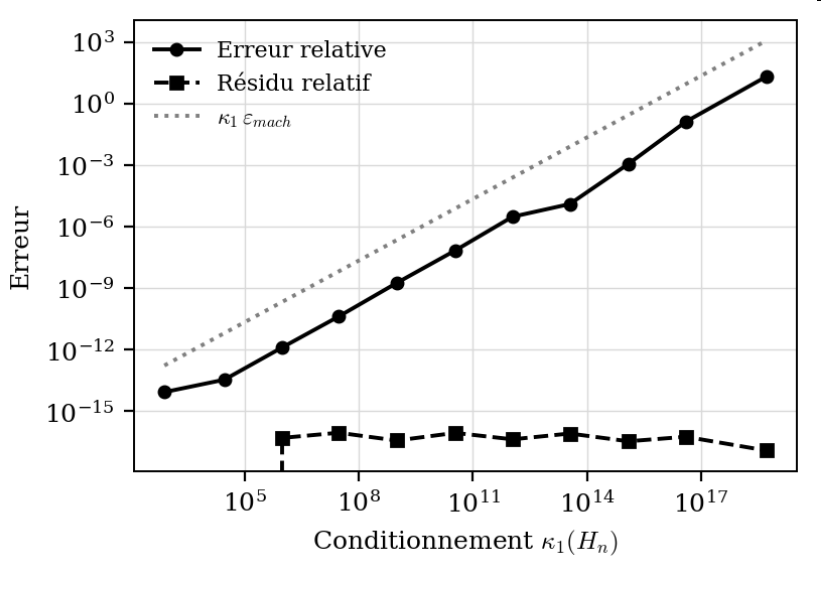
\includegraphics[width=\textwidth]{figures/fig3_hilbert.png}
    \caption{Matrices de Hilbert et \texttt{DGESV} : erreur et résidu en fonction de $\kappa_1(H_n)$.}
    \label{fig:fig3_hilbert}
\end{minipage}
\hfill
\begin{minipage}{0.48\textwidth}
    \centering
    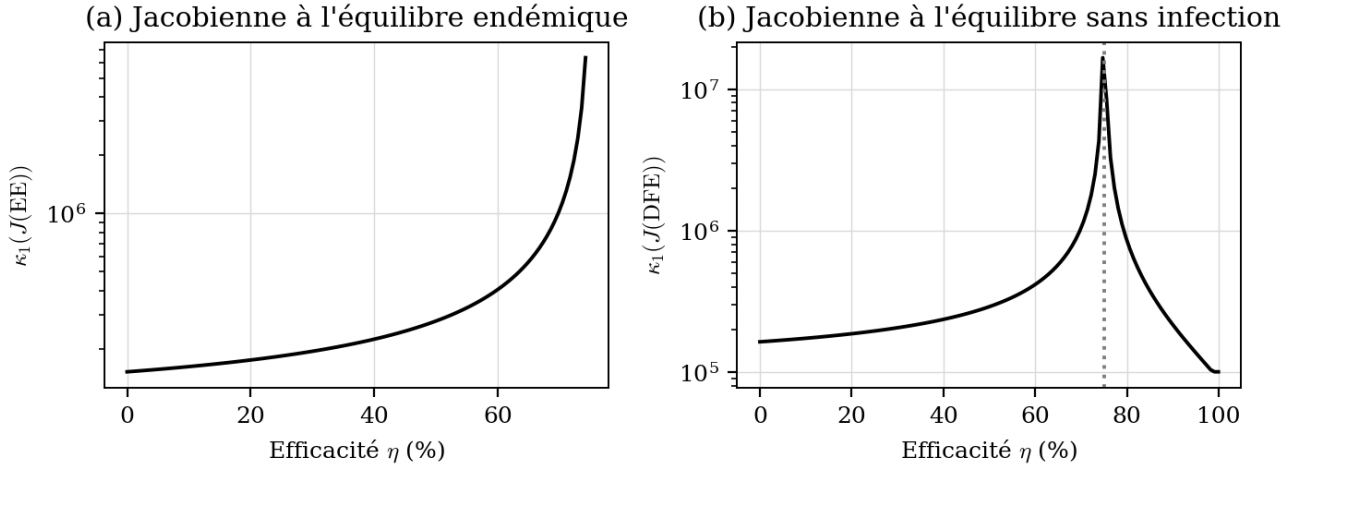
\includegraphics[width=\textwidth]{figures/fig4_cond_jac.png}
    \caption{Conditionnement $\kappa_1$ de la jacobienne en fonction de $\eta$.}
    \label{fig:fig4_cond_jac}
\end{minipage}
\end{figure}

\noindent\textbf{Lecture de la figure~\ref{fig:fig3_hilbert}.} L'erreur directe suit la droite $\kappa_1\varepsilon_{\mathrm{mach}}$ lorsque $\kappa_1$ croît, tandis que le résidu reste au niveau de la précision machine : \texttt{DGESV} fournit toujours une solution qui satisfait presque exactement le système, mais ne peut pas compenser un mauvais conditionnement du problème lui-même.

\noindent\textbf{Lecture de la figure~\ref{fig:fig4_cond_jac}.} La jacobienne du modèle est mal conditionnée à cause de la disparité des échelles ($T\sim10^3$ contre $V\sim10^2$--$10^4$, $p=1000$, $c=23$) : $\kappa_1(J(E^*))\approx1{,}5\times10^{5}$ pour $\eta=0$, et le conditionnement diverge lorsque l'on s'approche d'un point de bifurcation ($\eta\to\eta_c$).

\section{Équilibrage de la matrice jacobienne avec DGEEQU}

La routine \texttt{DGEEQU} calcule des coefficients diagonaux $R$ (lignes) et $C$ (colonnes) tels que $\widehat J=RJC$ ait des lignes et colonnes de normes comparables. Appliquée à la jacobienne du modèle :
\begin{center}
\begin{tabular}{lcc}
\toprule
\textbf{Point} & $\kappa_1(J)$ & $\kappa_1(RJC)$ \\
\midrule
Équilibre endémique $E^*$ ($\eta=0$) & $1{,}5\times10^{5}$ & $\approx 69$ \\
Équilibre sain $E_0$ ($\eta=0$) & $1{,}6\times10^{5}$ & $\approx 61$ \\
Pic de virémie (état $(60,300,17000)$) & $8{,}9\times10^{4}$ & $\approx 8$ \\
\bottomrule
\end{tabular}
\end{center}
L'équilibrage réduit donc le conditionnement de trois à quatre ordres de grandeur : il est indispensable avant toute inversion ou résolution quand les variables ont des unités et des échelles très différentes.

\section{Méthode de Newton avec DGESV et calcul spectral DGEEV}

Pour calculer un équilibre $f(y^*)=0$, on utilise la méthode de Newton :
$$J(y_k)\,\delta_k=-f(y_k),\qquad y_{k+1}=y_k+\delta_k ,$$
où le système $3\times3$ est résolu à chaque itération par \texttt{DGESV} (fonction \texttt{newton\_h}).

\begin{figure}[ht]
\centering
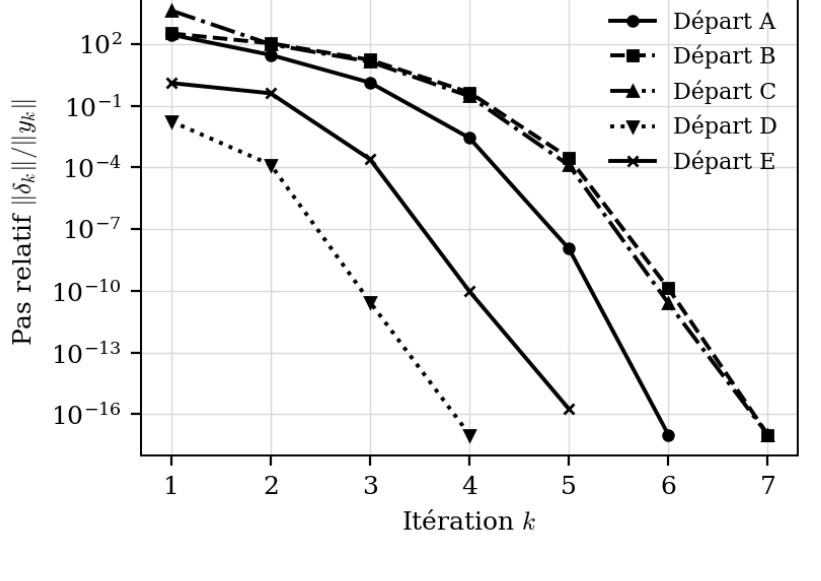
\includegraphics[width=0.55\textwidth]{figures/fig5_newton.png}
\caption{Convergence quadratique de la méthode de Newton (cinq points de départ).}
\label{fig:fig5_newton}
\end{figure}

\noindent\textbf{Lecture de la figure~\ref{fig:fig5_newton}.} L'axe vertical (échelle logarithmique) donne le pas relatif $\|\delta_k\|/\|y_k\|$. Depuis chacun des points de départ, la méthode converge en moins de dix itérations, avec la chute de plus en plus rapide du pas caractéristique de la convergence quadratique.

\medskip
Au point $E^*$, \texttt{DGEEV} fournit le spectre de la jacobienne donné au chapitre~6 : $\lambda_1=-23{,}50$ et $\lambda_{2,3}=-0{,}0197\pm0{,}1196\,i$. Le rapport $|\lambda_{\max}|/|\lambda_{\min}|\approx23{,}5/0{,}0197\approx1200$ quantifie la \emph{raideur} du système, étudiée au chapitre~8.

\begin{encadreresume}[Mini-résumé du chapitre 7 : solveurs LAPACK]
\begin{enumerate}
    \item \texttt{DGESV} donne un résidu au niveau de la précision machine ; l'erreur directe est limitée par $\kappa\,\varepsilon_{\mathrm{mach}}$.
    \item \texttt{DGEEQU} ramène $\kappa_1(J)$ d'environ $10^5$ à quelques dizaines.
    \item Newton + \texttt{DGESV} converge quadratiquement vers l'équilibre ; \texttt{DGEEV} en donne la stabilité.
\end{enumerate}
\end{encadreresume}

% ==============================================================================
% CHAPITRE 8 : INTÉGRATION NUMÉRIQUE
% ==============================================================================
\chapter{Intégration numérique des équations}

\section{Raideur et instabilité des schémas explicites}

\begin{cadreconcept}[Raideur (\textit{stiffness})]
Un système différentiel est dit \textbf{raide} lorsqu'il fait coexister des phénomènes d'échelles de temps très différentes. Ici : la clairance virale ($c=23$ j$^{-1}$, demi-vie de $43$ min) et la dynamique lente des CD4+ (échelle de $1/d=100$ j). Le rapport des valeurs propres extrêmes vaut environ $1200$.
\end{cadreconcept}

Pour le schéma d'\textbf{Euler explicite} $y_{k+1}=y_k+h f(y_k)$, la stabilité sur la composante rapide impose
$$h<\frac{2}{|\lambda_{\max}|}\approx\frac{2}{23{,}5}\approx0{,}085\ \text{jour}\ (\approx2\ \text{heures}).$$
Au-delà, les erreurs sont amplifiées à chaque pas : avec $h=0{,}1$ jour, notre simulation explicite déborde (valeurs non finies, dépassement de capacité des flottants) sur $30$ jours simulés, alors que le phénomène physique est parfaitement régulier (figure~\ref{fig:fig6_raideur}).

\begin{figure}[ht]
\centering
\begin{minipage}{0.48\textwidth}
    \centering
    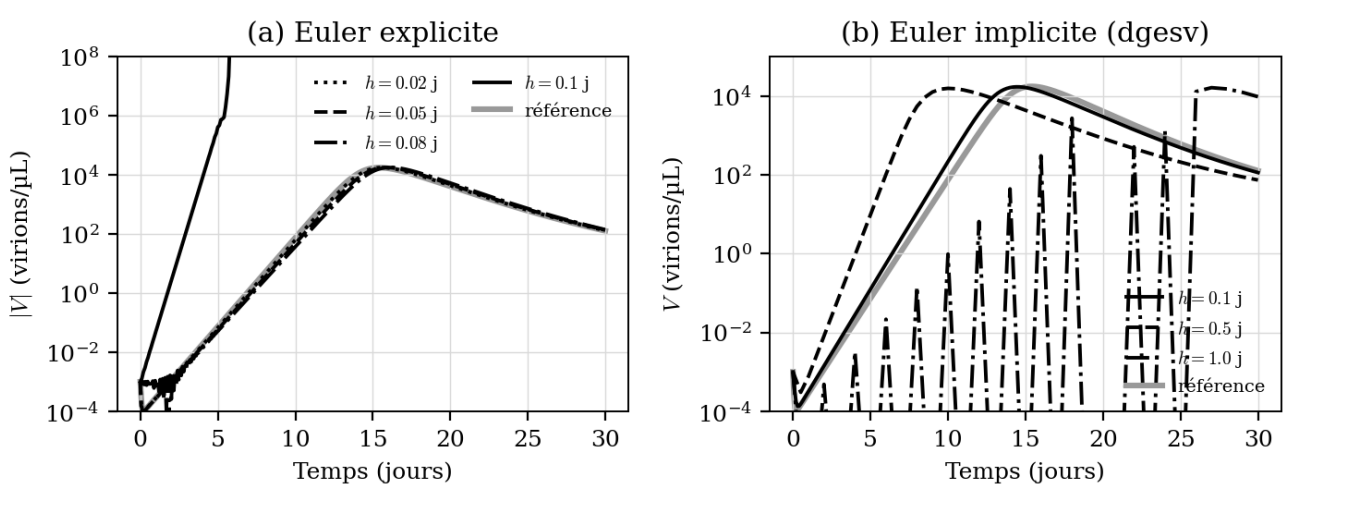
\includegraphics[width=\textwidth]{figures/fig6_raideur.png}
    \caption{Euler explicite (a) et Euler implicite (b) pour plusieurs pas $h$.}
    \label{fig:fig6_raideur}
\end{minipage}
\hfill
\begin{minipage}{0.48\textwidth}
    \centering
    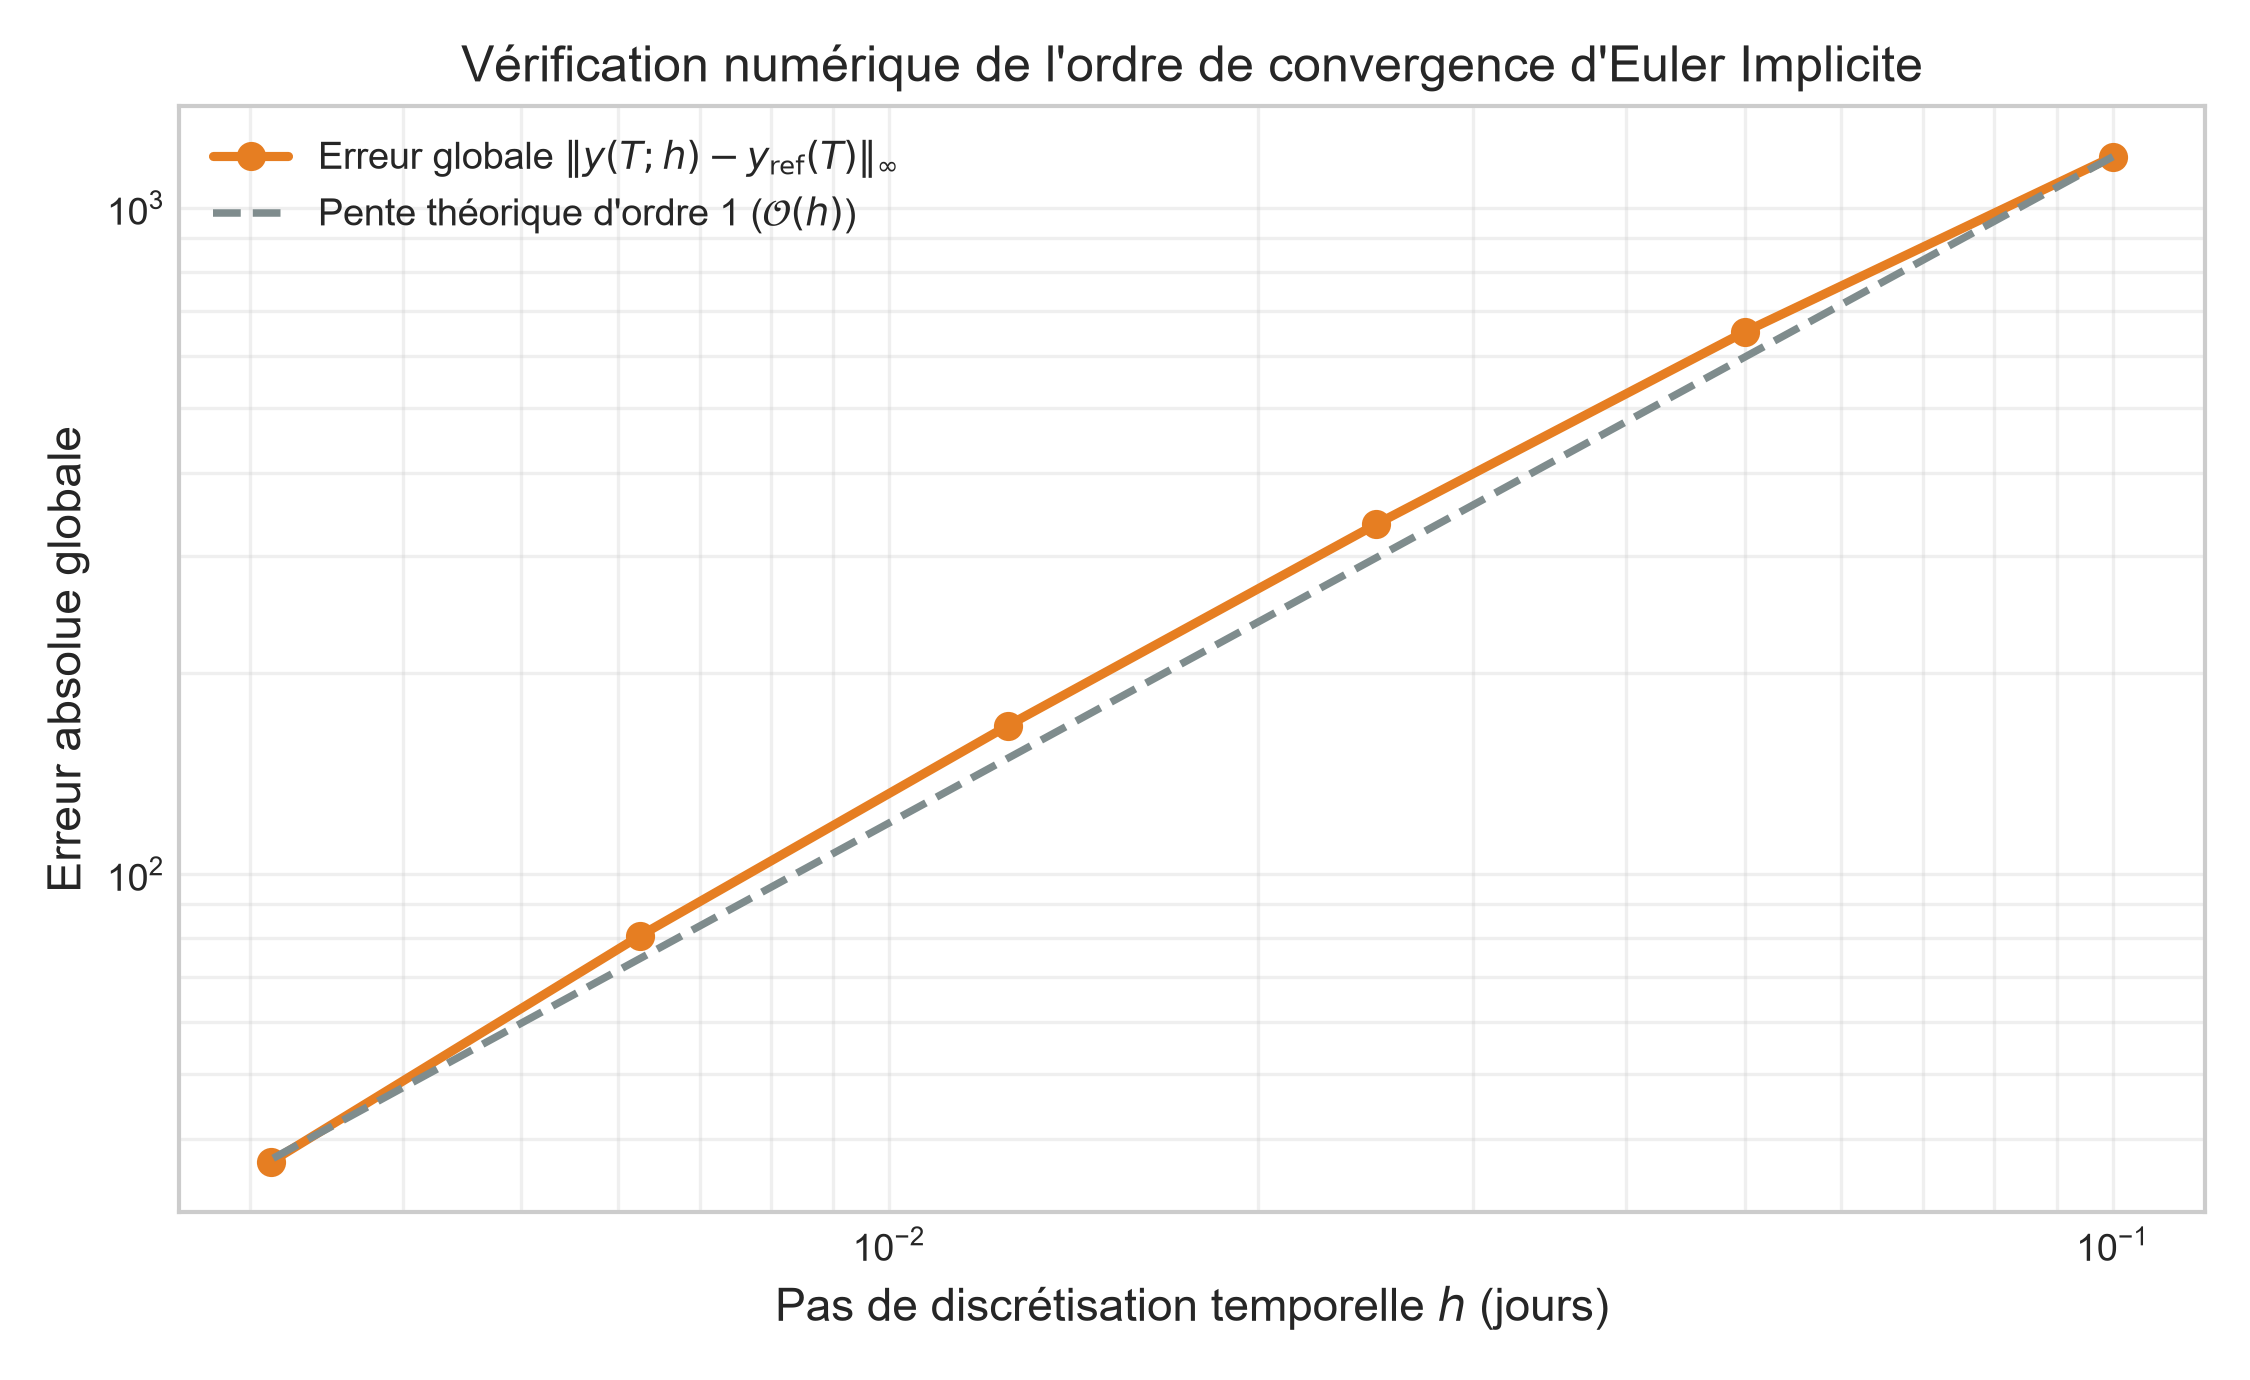
\includegraphics[width=\textwidth]{figures/fig7_convergence.png}
    \caption{Erreur à $t=10$ j en fonction du pas $h$.}
    \label{fig:fig7_convergence}
\end{minipage}
\end{figure}

\section{Schéma retenu et vérification}

\subsection*{Le schéma d'Euler implicite linéarisé}

Pour s'affranchir de la contrainte de stabilité, nous retenons l'\textbf{Euler implicite} $y_{k+1}=y_k+hf(y_{k+1})$, linéarisé autour de $y_k$ (une itération de Newton par pas) :
\begin{equation}
\big[I-h\,J(y_k)\big]\,\Delta y_k=h\,f(y_k),\qquad y_{k+1}=y_k+\Delta y_k .
\label{eq:euler_implicite}
\end{equation}
À chaque pas, le système linéaire $3\times3$ est résolu par \texttt{DGESV}. Sur un problème linéaire $\dot y=\lambda y$, ce schéma est A-stable : le facteur d'amplification $1/(1-h\lambda)$ est de module inférieur à $1$ pour tout $h>0$ et $\mathrm{Re}\,\lambda<0$, quelle que soit la raideur. Il est d'ordre $1$. Une projection sur l'orthant positif ($y\leftarrow\max(y,0)$) est appliquée pour garantir la positivité numérique. Le choix est motivé par la simplicité, la robustesse et le recours naturel à LAPACK ; pour une précision supérieure on utiliserait un schéma d'ordre plus élevé (Radau, BDF)~\cite{hairer1996}.

\subsection*{Protocole de vérification}

Nous vérifions le schéma selon trois critères, avec $y(0)=(1000,\,0,\,10^{-3})$ et $\eta=0$. La solution de référence est calculée avec le solveur implicite d'ordre élevé \texttt{Radau} (SciPy, tolérances $10^{-12}$).

\paragraph{(i) Stabilité.} À $h=0{,}1$ jour, Euler explicite diverge (valeurs non finies avant $30$ jours), tandis qu'Euler implicite reste borné et reproduit la phase de pic viral. Le schéma implicite reste stable même pour $h=0{,}5$ et $h=1$ jour (figure~\ref{fig:fig6_raideur}b), au prix d'un décalage temporel du pic.

\paragraph{(ii) Convergence.} Le tableau~\ref{tab:verif_ordre} donne l'erreur relative (norme euclidienne des erreurs relatives par composante) sur $[0,10]$ jours et l'ordre observé $p\approx\log_2(e_h/e_{h/2})$.

\begin{table}[ht]
\centering
\caption{Erreur du schéma d'Euler implicite à $t=10$ j par rapport à la solution de référence.}
\label{tab:verif_ordre}
\begin{tabular}{c c c}
\toprule
\textbf{Pas $h$ (jour)} & \textbf{Erreur relative} & \textbf{Ordre observé} \\
\midrule
$0{,}4$ & $2{,}3\times10^{2}$ & -- \\
$0{,}2$ & $13$ & $4{,}1$ \\
$0{,}1$ & $2{,}6$ & $2{,}3$ \\
$0{,}05$ & $0{,}92$ & $1{,}5$ \\
$0{,}025$ & $0{,}39$ & $1{,}2$ \\
$0{,}0125$ & $0{,}18$ & $1{,}1$ \\
\bottomrule
\end{tabular}
\end{table}

L'ordre observé tend vers $1$ lorsque $h$ diminue, conformément à la théorie. Les erreurs absolues restent élevées aux grands pas parce que $t=10$ j se situe en pleine croissance exponentielle du virus ($V$ est multiplié par un facteur voisin de $e^{c\cdot\mathrm{croissance}}$ sur quelques jours), phase où l'erreur d'un schéma d'ordre $1$ est amplifiée ; cela confirme qu'un pas $h\le0{,}0125$ j (ou un schéma d'ordre supérieur) est nécessaire pour une précision quantitative sur la primo-infection.

\paragraph{(iii) Cohérence asymptotique.} Un point fixe du schéma~\eqref{eq:euler_implicite} est exactement un équilibre de $f$ (car $f(y)=0$ donne $\Delta y=0$). Nous l'avons vérifié : avec $h=0{,}1$ jour, la solution à $t=600$ j coïncide avec $E^*=(250;\,15;\,652{,}17)$ à $2\times10^{-5}$ près en erreur relative, écart dû uniquement à la décroissance lente de l'oscillation résiduelle ($e^{-0{,}0197\,t}$). Les équilibres calculés par Newton (section~7.3) et par intégration en temps long sont donc cohérents.

\begin{encadreresume}[Mini-résumé du chapitre 8 : intégration numérique]
\begin{enumerate}
    \item Le système est raide (rapport des valeurs propres $\approx1200$) ; Euler explicite exige $h<0{,}085$ j et diverge à $h=0{,}1$ j.
    \item Le schéma retenu est l'Euler implicite linéarisé résolu par \texttt{DGESV}, stable sans contrainte sur $h$.
    \item Vérification : ordre observé $\to1$, stabilité à grands pas, point fixe $=$ équilibre.
    \item Précision quantitative : pas fin ou schéma d'ordre supérieur.
\end{enumerate}
\end{encadreresume}

% ==============================================================================
% CHAPITRE 9 : RÉSULTATS
% ==============================================================================
\chapter{Résultats et interprétation médicale}

\section{Primo-infection et portrait de phase}

Partant de $T=1000$ (sujet sain), $I=0$ et d'une trace de virus $V=10^{-3}$ virion/$\mu$L, la simulation du modèle non traité (figure~\ref{fig:fig8_infection}) montre :
\begin{itemize}
    \item un \textbf{pic de virémie} d'environ $1{,}7\times10^{4}$ virions/$\mu$L atteint vers le jour $15$ ;
    \item une \textbf{chute transitoire des CD4+} jusqu'à environ $49$ cellules/$\mu$L ;
    \item puis des oscillations amorties (période $\approx53$ j) vers l'équilibre chronique $E^*=(250,\,15,\,652)$.
\end{itemize}

\begin{figure}[ht]
\centering
\begin{minipage}{0.48\textwidth}
    \centering
    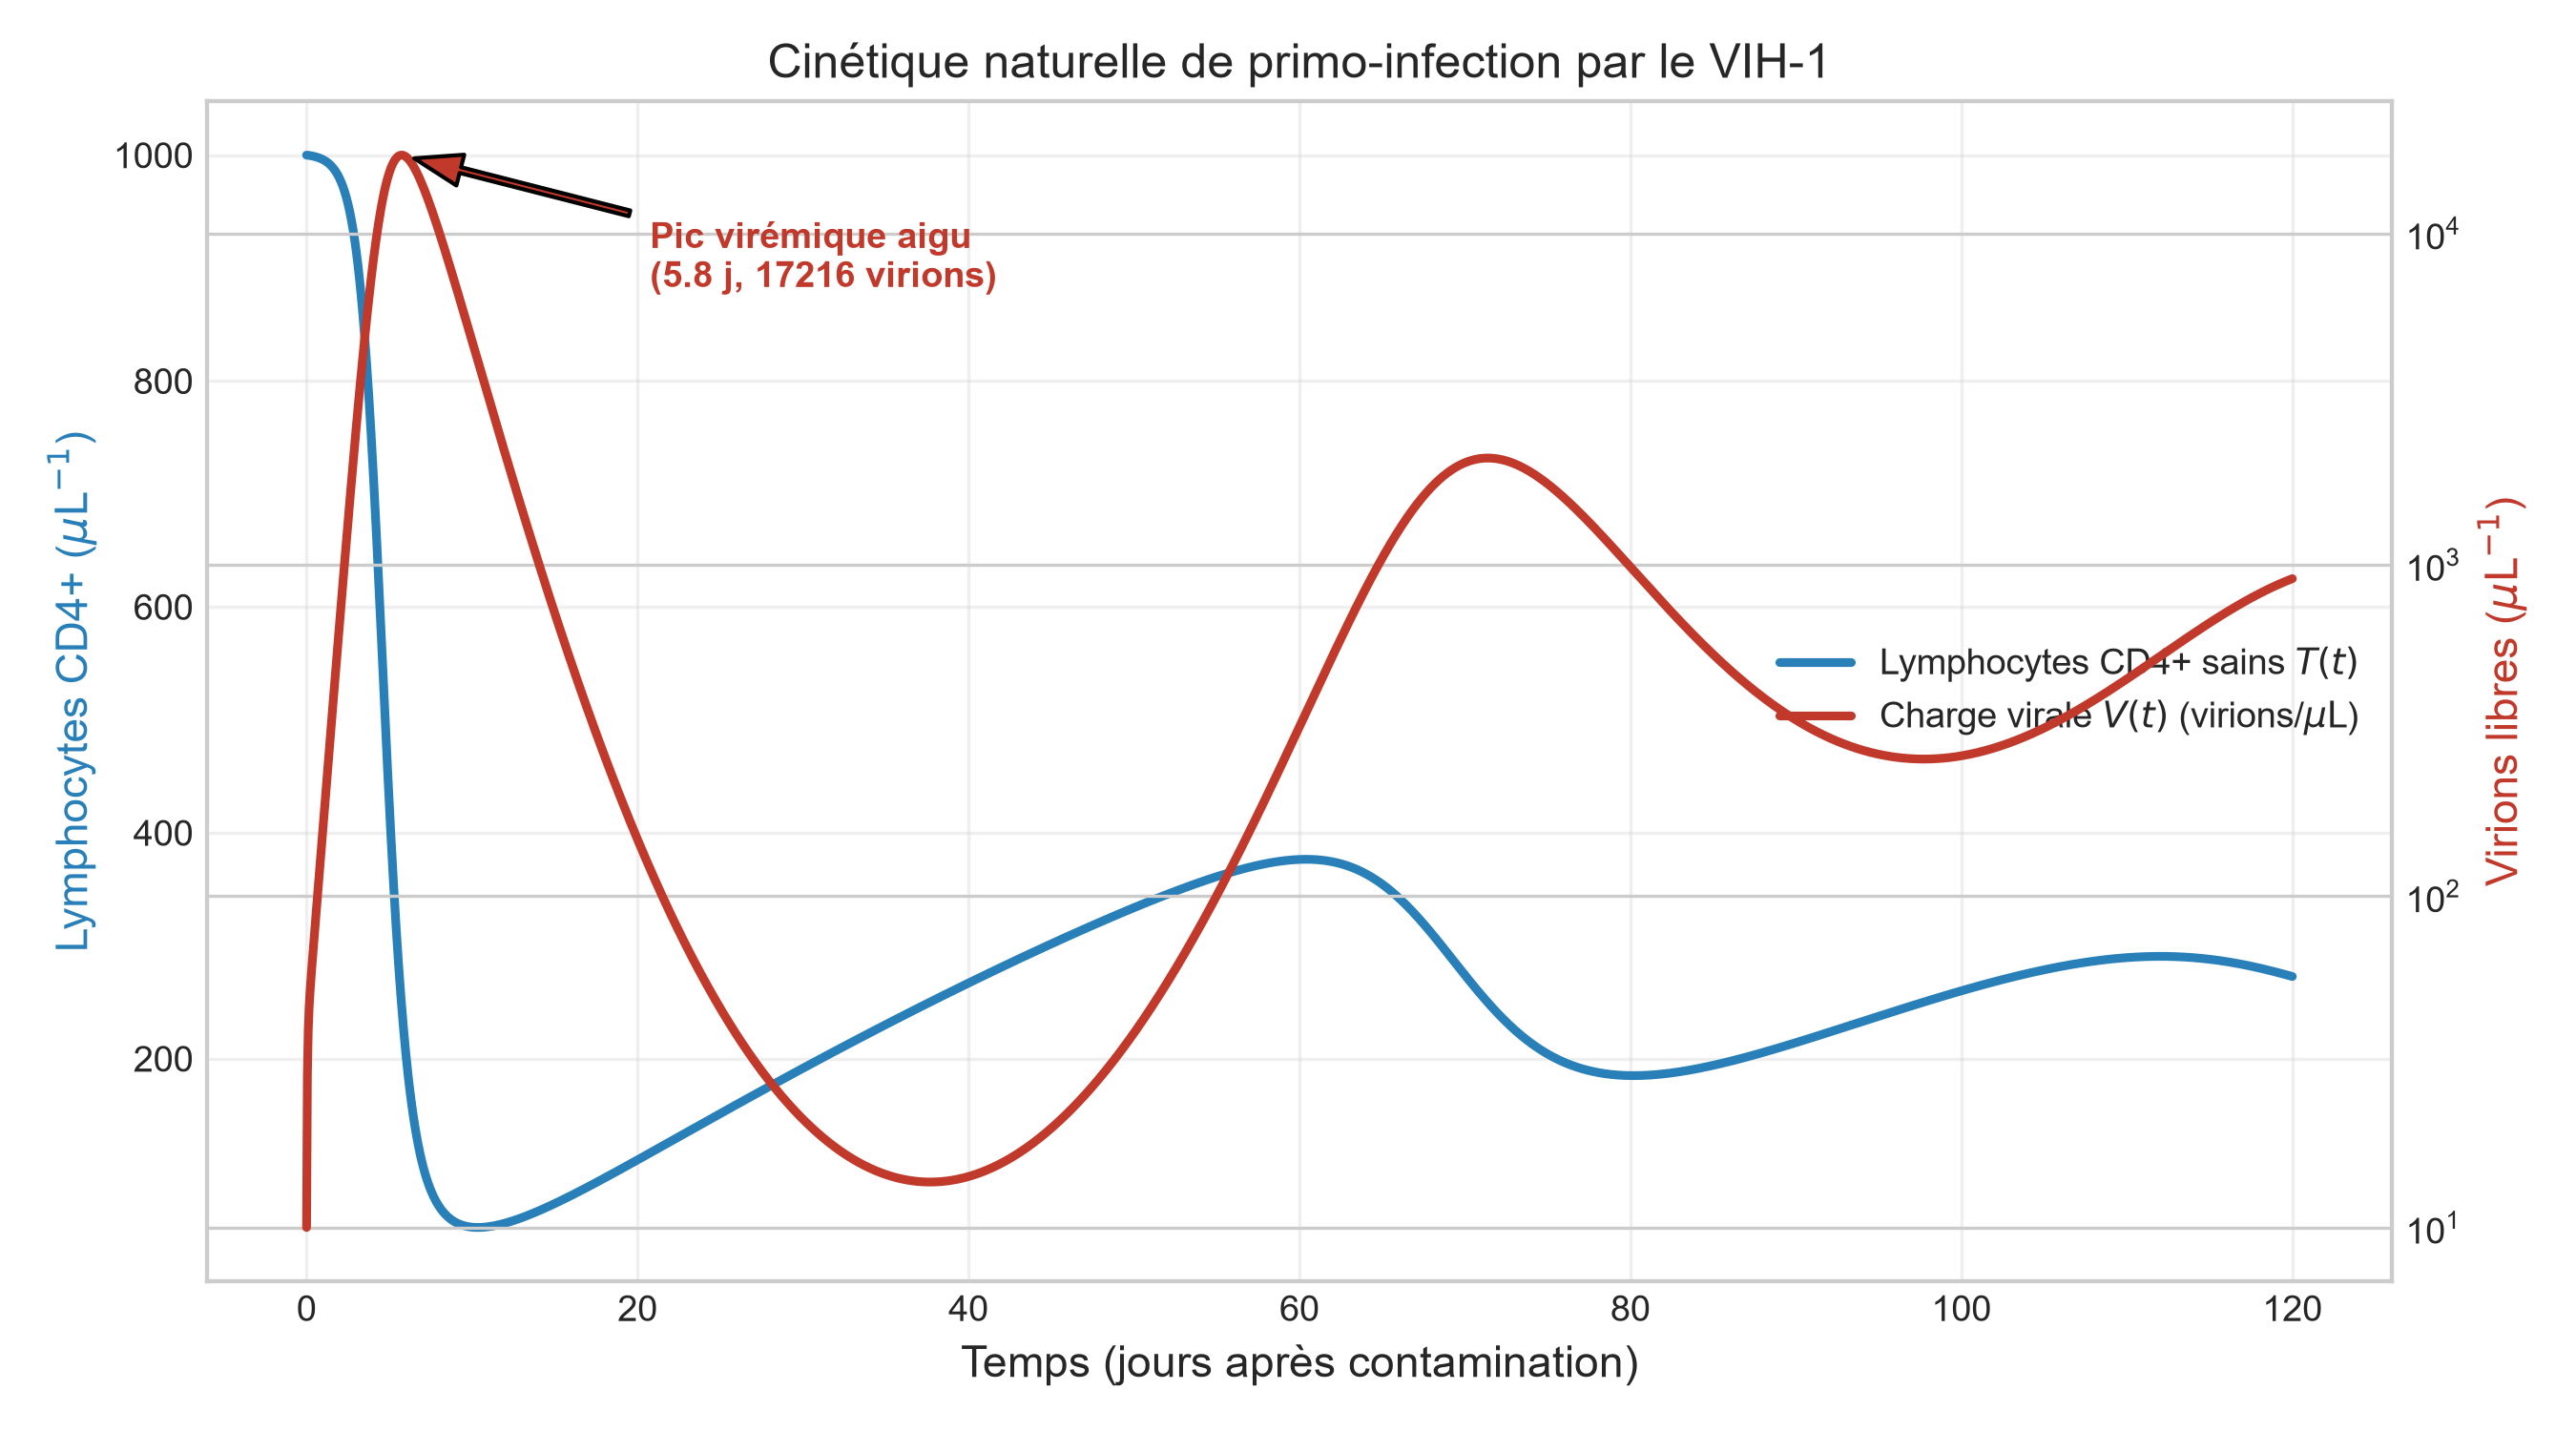
\includegraphics[width=\textwidth]{figures/fig8_infection_primaire.png}
    \caption{Primo-infection : $T(t)$, $I(t)$ et $V(t)$.}
    \label{fig:fig8_infection}
\end{minipage}
\hfill
\begin{minipage}{0.48\textwidth}
    \centering
    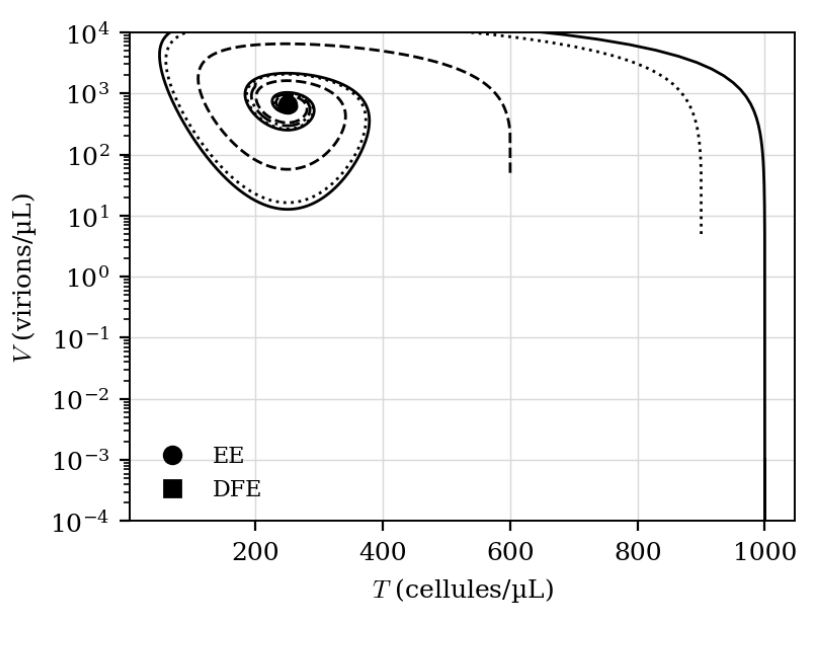
\includegraphics[width=\textwidth]{figures/fig9_portrait_phase.png}
    \caption{Portrait de phase $(T,V)$ depuis plusieurs conditions initiales.}
    \label{fig:fig9_phase}
\end{minipage}
\end{figure}

\noindent\textbf{Interprétation.} Le pic viral massif suivi d'un déclin est la signature de la phase aiguë : le virus consomme brutalement les cellules cibles, puis il est limité par leur raréfaction. Sur la figure~\ref{fig:fig9_phase}, toutes les trajectoires s'enroulent en spirale vers un même point $E^*$, ce qui illustre la stabilité globale de l'équilibre endémique pour $\Rzero>1$.

\section{Efficacité thérapeutique et rebond viral}

\paragraph{Seuil d'efficacité.} Pour $\eta=50\,\%$, $70\,\%$ et $95\,\%$, on obtient $\Rzero=2{,}0$, $1{,}2$ et $0{,}2$. Seul le dernier cas conduit à l'élimination du virus (figure~\ref{fig:fig10_r0_eta}). En partant de l'équilibre chronique et avec $\eta=95\,\%$, la charge virale passe sous le seuil d'indétectabilité de $0{,}05$ virion/$\mu$L en environ $20$ jours et les CD4+ remontent (environ $900$/$\mu$L après $200$ jours). Pour $\eta=70\,\%$, la charge virale passe elle aussi sous ce seuil (en environ $34$ jours) et descend jusqu'à $\approx10^{-6}$ virion/$\mu$L, mais ce n'est qu'un \emph{répit} : comme $\Rzero=1{,}2>1$, le virus n'est pas éliminé et remonte lentement (en plusieurs centaines de jours) vers un équilibre endémique à $\approx145$ virions/$\mu$L. À $\eta=50\,\%$, la charge virale diminue transitoirement puis \emph{rebondit} en oscillant vers un équilibre à $\approx435$ virions/$\mu$L. Une charge virale indétectable n'est donc pas une preuve de guérison tant que $\eta<\eta_c$.

\begin{figure}[ht]
\centering
\begin{minipage}{0.48\textwidth}
    \centering
    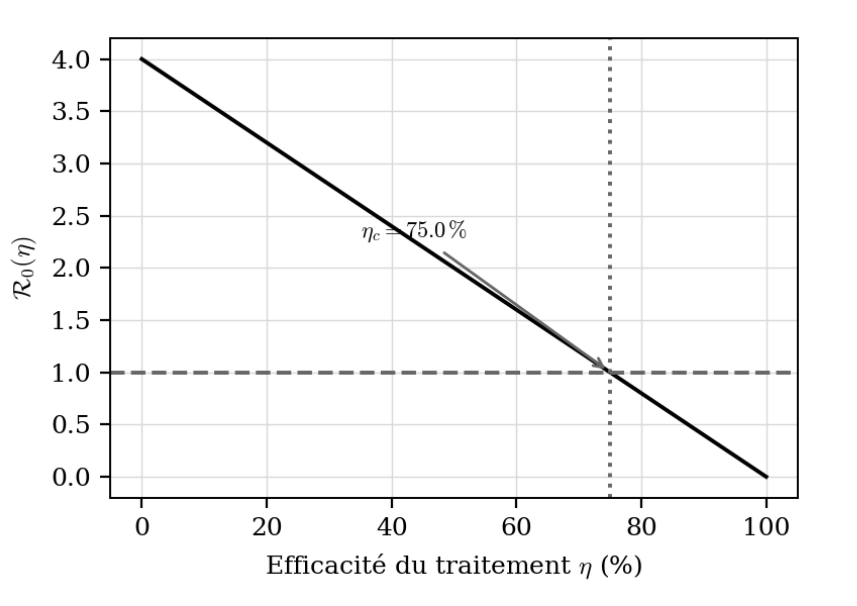
\includegraphics[width=\textwidth]{figures/fig10_r0_eta.png}
    \caption{$\Rzero$ en fonction de l'efficacité $\eta$.}
    \label{fig:fig10_r0_eta}
\end{minipage}
\hfill
\begin{minipage}{0.48\textwidth}
    \centering
    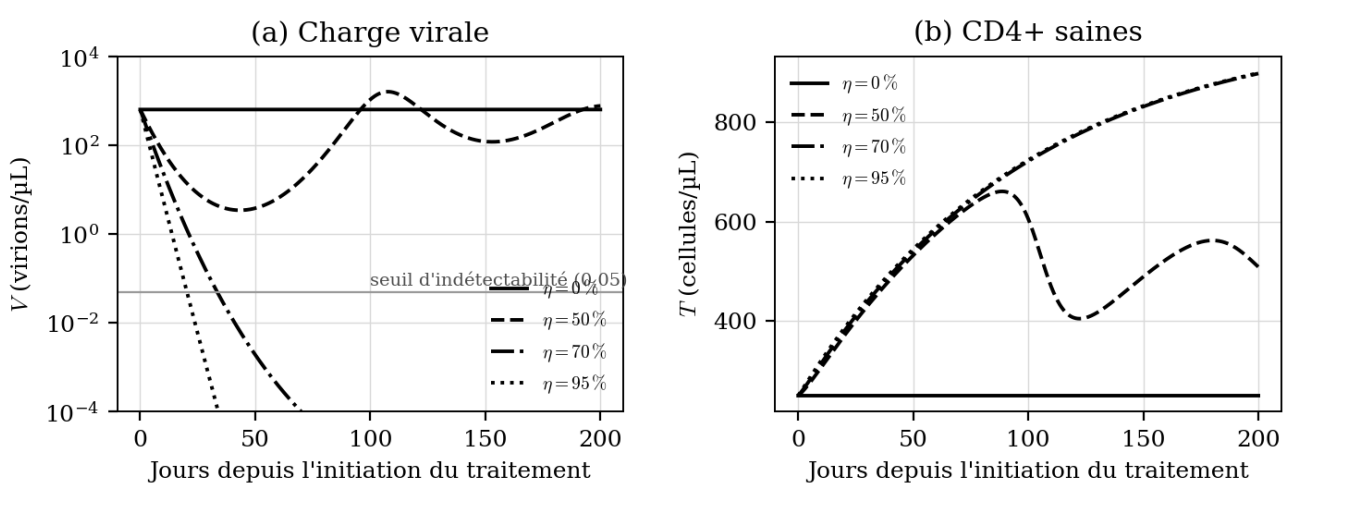
\includegraphics[width=\textwidth]{figures/fig11_traitement.png}
    \caption{Charge virale (a) et CD4+ (b) pour plusieurs efficacités $\eta$.}
    \label{fig:fig11_traitement}
\end{minipage}
\end{figure}

\paragraph{Bifurcation et sensibilité.} La figure~\ref{fig:fig12_bifurcation} représente les équilibres $T^*,I^*,V^*$ en fonction de $\Rzero$ : à $\Rzero=1$, $E_0$ et $E^*$ échangent leur stabilité (bifurcation transcritique). La figure~\ref{fig:fig14_sensibilite} montre les indices de sensibilité normalisés $\Upsilon_q^{\Rzero}=\frac{\partial\Rzero}{\partial q}\frac q{\Rzero}$ :
$$\Upsilon^{\Rzero}_{\beta}=\Upsilon^{\Rzero}_{p}=\Upsilon^{\Rzero}_{s}=+1,\qquad \Upsilon^{\Rzero}_{d}=\Upsilon^{\Rzero}_{\delta}=\Upsilon^{\Rzero}_{c}=-1,$$
puisque $\Rzero$ est un monôme en les paramètres. Une variation de $1\,\%$ de $\beta$, $p$ ou $s$ modifie $\Rzero$ de $+1\,\%$ ; celle de $d$, $\delta$ ou $c$ de $-1\,\%$. Pour la charge virale d'équilibre, nous trouvons $\Upsilon^{V^*}_{s}=\Upsilon^{V^*}_{p}=+4/3$, $\Upsilon^{V^*}_{\delta}=\Upsilon^{V^*}_{c}=-4/3$, $\Upsilon^{V^*}_{\beta}=+1/3$, $\Upsilon^{V^*}_{d}=-1/3$ : l'infectivité $\beta$ influence $\Rzero$ mais bien moins la charge virale chronique.

\begin{figure}[ht]
\centering
\begin{minipage}{0.48\textwidth}
    \centering
    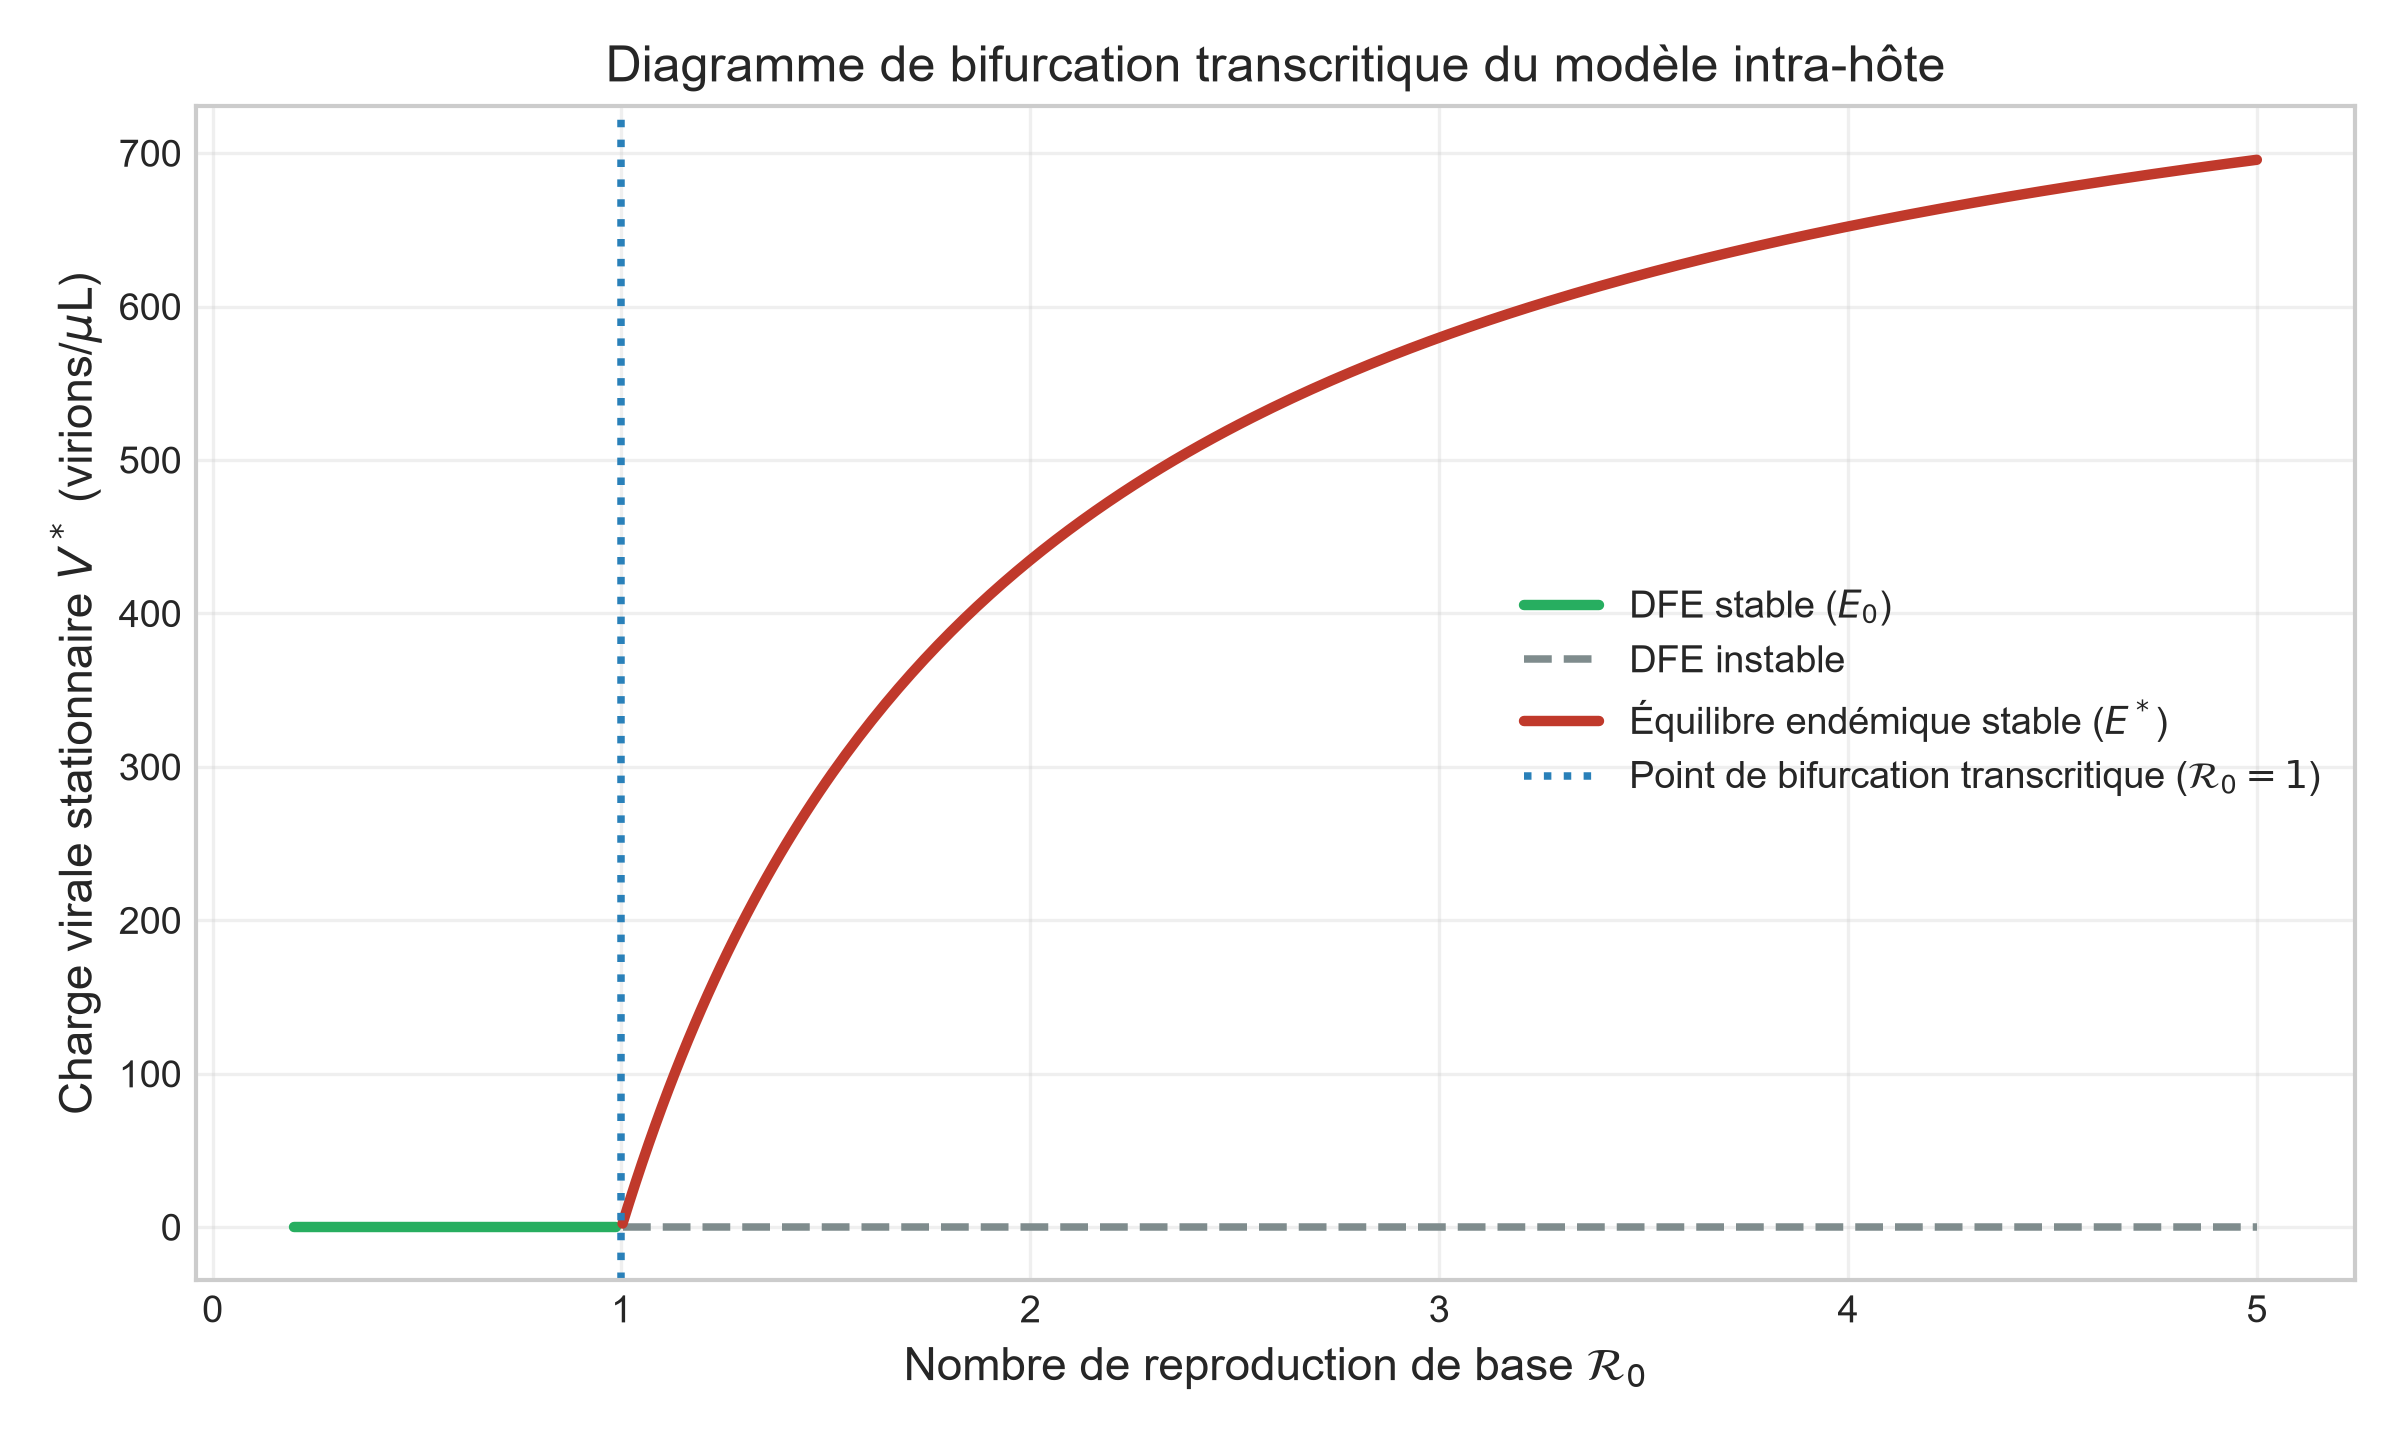
\includegraphics[width=\textwidth]{figures/fig12_bifurcation_intra.png}
    \caption{Bifurcation transcritique à $\Rzero=1$ et échange de stabilité.}
    \label{fig:fig12_bifurcation}
\end{minipage}
\hfill
\begin{minipage}{0.48\textwidth}
    \centering
    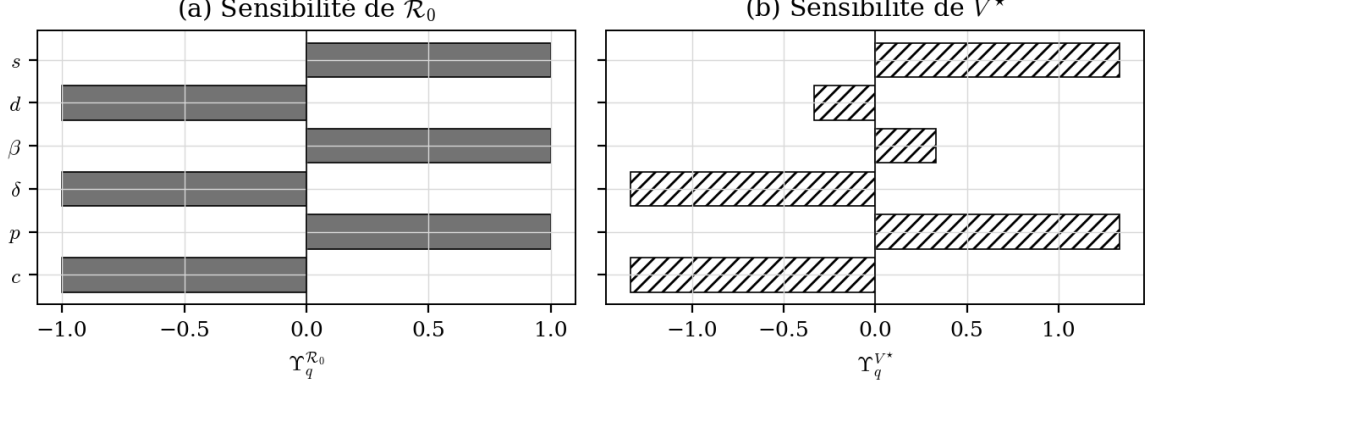
\includegraphics[width=\textwidth]{figures/fig14_sensibilite.png}
    \caption{Indices de sensibilité de $\Rzero$ et de $V^*$.}
    \label{fig:fig14_sensibilite}
\end{minipage}
\end{figure}

\paragraph{Danger de l'interruption du traitement.} Pour un patient traité à $\eta=95\,\%$ jusqu'au jour $100$ puis \emph{sans traitement}, le stock de CD4+ s'est reconstitué ($T\approx724$ cellules/$\mu$L au jour $100$) alors que la charge virale est indétectable. À l'arrêt, le virus résiduel dispose de ces cellules cibles abondantes : la charge virale subit un \textbf{rebond} d'un pic d'environ $1{,}2\times10^{4}$ virions/$\mu$L (jour $\approx150$), soit environ \textbf{$18$ fois le niveau chronique} ($652$), avant de retourner vers $E^*$ en oscillant (figure~\ref{fig:fig13_amplif}). Ce phénomène est une \emph{amplification transitoire} : bien que $E^*$ soit stable, des trajectoires partant d'un état très éloigné croissent fortement avant de décroître. Il justifie l'exigence d'une observance continue du traitement.

\begin{figure}[ht]
\centering
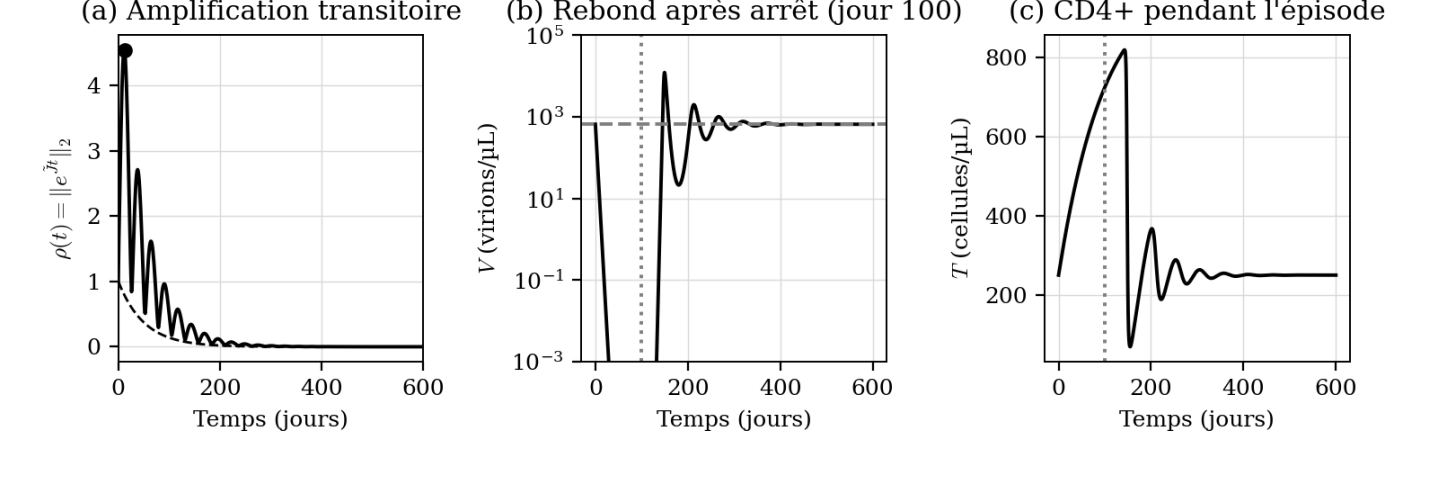
\includegraphics[width=0.95\textwidth]{figures/fig13_amplification.png}
\caption{Amplification transitoire et rebond viral après arrêt du traitement.}
\label{fig:fig13_amplif}
\end{figure}

\begin{encadreresume}[Mini-résumé du chapitre 9 : interprétation médicale]
\begin{enumerate}
    \item La primo-infection produit un pic de virémie ($\approx1{,}7\times10^{4}$) et un effondrement transitoire des CD4+.
    \item Il faut $\eta>75\,\%$ pour éradiquer le virus ; $\eta=95\,\%$ rend la charge virale indétectable en $\approx20$ jours.
    \item L'arrêt du traitement provoque un rebond viral d'environ $18$ fois le niveau chronique.
    \item $\Rzero$ est également sensible à $s,\beta,p$ ($+1$) et à $d,\delta,c$ ($-1$).
\end{enumerate}
\end{encadreresume}

% ==============================================================================
% CHAPITRE 10 : MODÈLE DE POPULATION
% ==============================================================================
\chapter{Modèle épidémiologique de population : $S, I_1, I_2$}

\section{Formulation du modèle de population}

À l'échelle d'une communauté, la population $N(t)$ est divisée en trois groupes :
\begin{itemize}
    \item $S(t)$ : individus sains, susceptibles d'être infectés ;
    \item $I_1(t)$ : personnes infectées par le VIH, contagieuses mais sans symptômes ;
    \item $I_2(t)$ : personnes au stade SIDA.
\end{itemize}
Le modèle s'écrit
\begin{equation}
\begin{cases}
\dfrac{dS}{dt}=\Lambda_aN-\beta S\dfrac{I_1+\varepsilon I_2}{N}-\mu_aS\\[10pt]
\dfrac{dI_1}{dt}=\beta S\dfrac{I_1+\varepsilon I_2}{N}-\sigma I_1-\mu_aI_1\\[10pt]
\dfrac{dI_2}{dt}=\sigma I_1-\mu_2I_2-\mu_aI_2
\end{cases}
\label{eq:pop_modele}
\end{equation}
avec $N=S+I_1+I_2$, $\Lambda_a$ le taux de natalité, $\mu_a$ la mortalité naturelle, $\sigma$ le taux de progression vers le SIDA, $\mu_2$ la surmortalité liée au SIDA et $\varepsilon<1$ la contagiosité relative au stade SIDA.

\begin{figure}[ht]
\centering
\begin{tikzpicture}[
    node distance=2.8cm,
    compartment/.style={rectangle, draw=navyblue, fill=lightbg, thick, minimum width=2.4cm, minimum height=1.1cm, align=center, font=\small\bfseries},
    rate/.style={->, >=stealth, thick, color=navyblue}
]
    \node (birth) {};
    \node[compartment, right=1.2cm of birth] (S) {S\\{\footnotesize Susceptibles}};
    \node[compartment, right=of S] (I1) {$I_1$\\{\footnotesize Infectés VIH}};
    \node[compartment, right=of I1] (I2) {$I_2$\\{\footnotesize Stade SIDA}};
    \node[below=1.2cm of S] (sinkS) {};
    \node[below=1.2cm of I1] (sinkI1) {};
    \node[below=1.2cm of I2] (sinkI2) {};
    \draw[rate] (birth) -- node[above]{\small $\Lambda_a N$} (S);
    \draw[rate] (S) -- node[below]{\small $\mu_a S$} (sinkS);
    \draw[rate] (S) -- node[above]{\small $\beta S \frac{I_1+\varepsilon I_2}{N}$} (I1);
    \draw[rate] (I1) -- node[below]{\small $\mu_a I_1$} (sinkI1);
    \draw[rate] (I1) -- node[above]{\small $\sigma I_1$} (I2);
    \draw[rate] (I2) -- node[below]{\small $(\mu_2 + \mu_a)I_2$} (sinkI2);
\end{tikzpicture}
\caption{Schéma de transfert du modèle de population $S$--$I_1$--$I_2$.}
\label{fig:tikz_transfert_pop}
\end{figure}

\begin{cadreconcept}[Pourquoi diviser par $N$ dans le terme d'infection ?]
Dans les infections sexuellement transmissibles, le nombre de partenaires d'un individu ne dépend pas de la taille de la population. L'incidence est donc \textbf{standardisée} : $\beta S\frac{I_1+\varepsilon I_2}{N}$ ($\beta$ est le taux de contact efficace par individu), et non proportionnelle à $N$ (action de masse).
\end{cadreconcept}

\paragraph{Passage aux proportions.} Posons $s=S/N$, $i_1=I_1/N$, $i_2=I_2/N$ avec $s=1-i_1-i_2$. Comme $N'/N=\Lambda_a-\mu_a-\mu_2\,i_2$, le système se réduit à deux équations (implémentées par \texttt{f\_B} dans le code) :
\begin{align*}
i_1'&=\beta\,s\,(i_1+\varepsilon i_2)-(\sigma+\Lambda_a)\,i_1+\mu_2\,i_1i_2,\\
i_2'&=\sigma i_1-(\mu_2+\Lambda_a)\,i_2+\mu_2\,i_2^{\,2}.
\end{align*}

\section{Nombre de reproduction de base et équilibres}

Au point sans maladie ($s=1$), on applique la même méthode qu'au chapitre~6 aux variables infectées $(i_1,i_2)$ : $F$ contient les \emph{nouvelles infections} et $V_m$ les \emph{passages et sorties} (progression vers le SIDA, mortalité). On obtient
$$F=\begin{pmatrix}\beta&\beta\varepsilon\\0&0\end{pmatrix},\quad V_m=\begin{pmatrix}\sigma+\Lambda_a&0\\-\sigma&\mu_2+\Lambda_a\end{pmatrix}\ \Longrightarrow\
\boxed{\ \Rzero^{\mathrm{pop}}=\frac{\beta}{\sigma+\Lambda_a}\Big(1+\frac{\varepsilon\sigma}{\mu_2+\Lambda_a}\Big)\ }$$
Les deux termes s'interprètent comme la contribution d'un individu $I_1$ pendant sa phase asymptomatique, puis pendant sa phase SIDA (affaiblie d'un facteur $\varepsilon$). Avec les valeurs calibrées $\Lambda_a=0{,}04$, $\sigma=0{,}10$, $\mu_2=0{,}50$, $\varepsilon=0{,}30$ et $\beta=0{,}2387$ (choisi pour obtenir $\Rzero^{\mathrm{pop}}=1{,}8$), on a $\Rzero^{\mathrm{pop}}=1{,}8$. Le seuil critique est
$$\beta_c=\frac{\sigma+\Lambda_a}{1+\varepsilon\sigma/(\mu_2+\Lambda_a)}\approx0{,}133 .$$
Pour $\Rzero^{\mathrm{pop}}>1$, le système converge vers un équilibre endémique stable d'environ $s^*=32{,}2\,\%$, $i_1^*=56{,}1\,\%$, $i_2^*=11{,}6\,\%$, soit une \textbf{prévalence} totale de $67{,}8\,\%$ ; la jacobienne réduite en ce point a pour valeurs propres $-0{,}098$ et $-0{,}473$ (réelles et négatives : l'approche est monotone, sans oscillation). Partant d'une faible prévalence initiale, la moitié de la valeur de plateau est atteinte vers l'année $59$ et $90\,\%$ vers l'année $81$.

\begin{figure}[ht]
\centering
\begin{minipage}{0.48\textwidth}
    \centering
    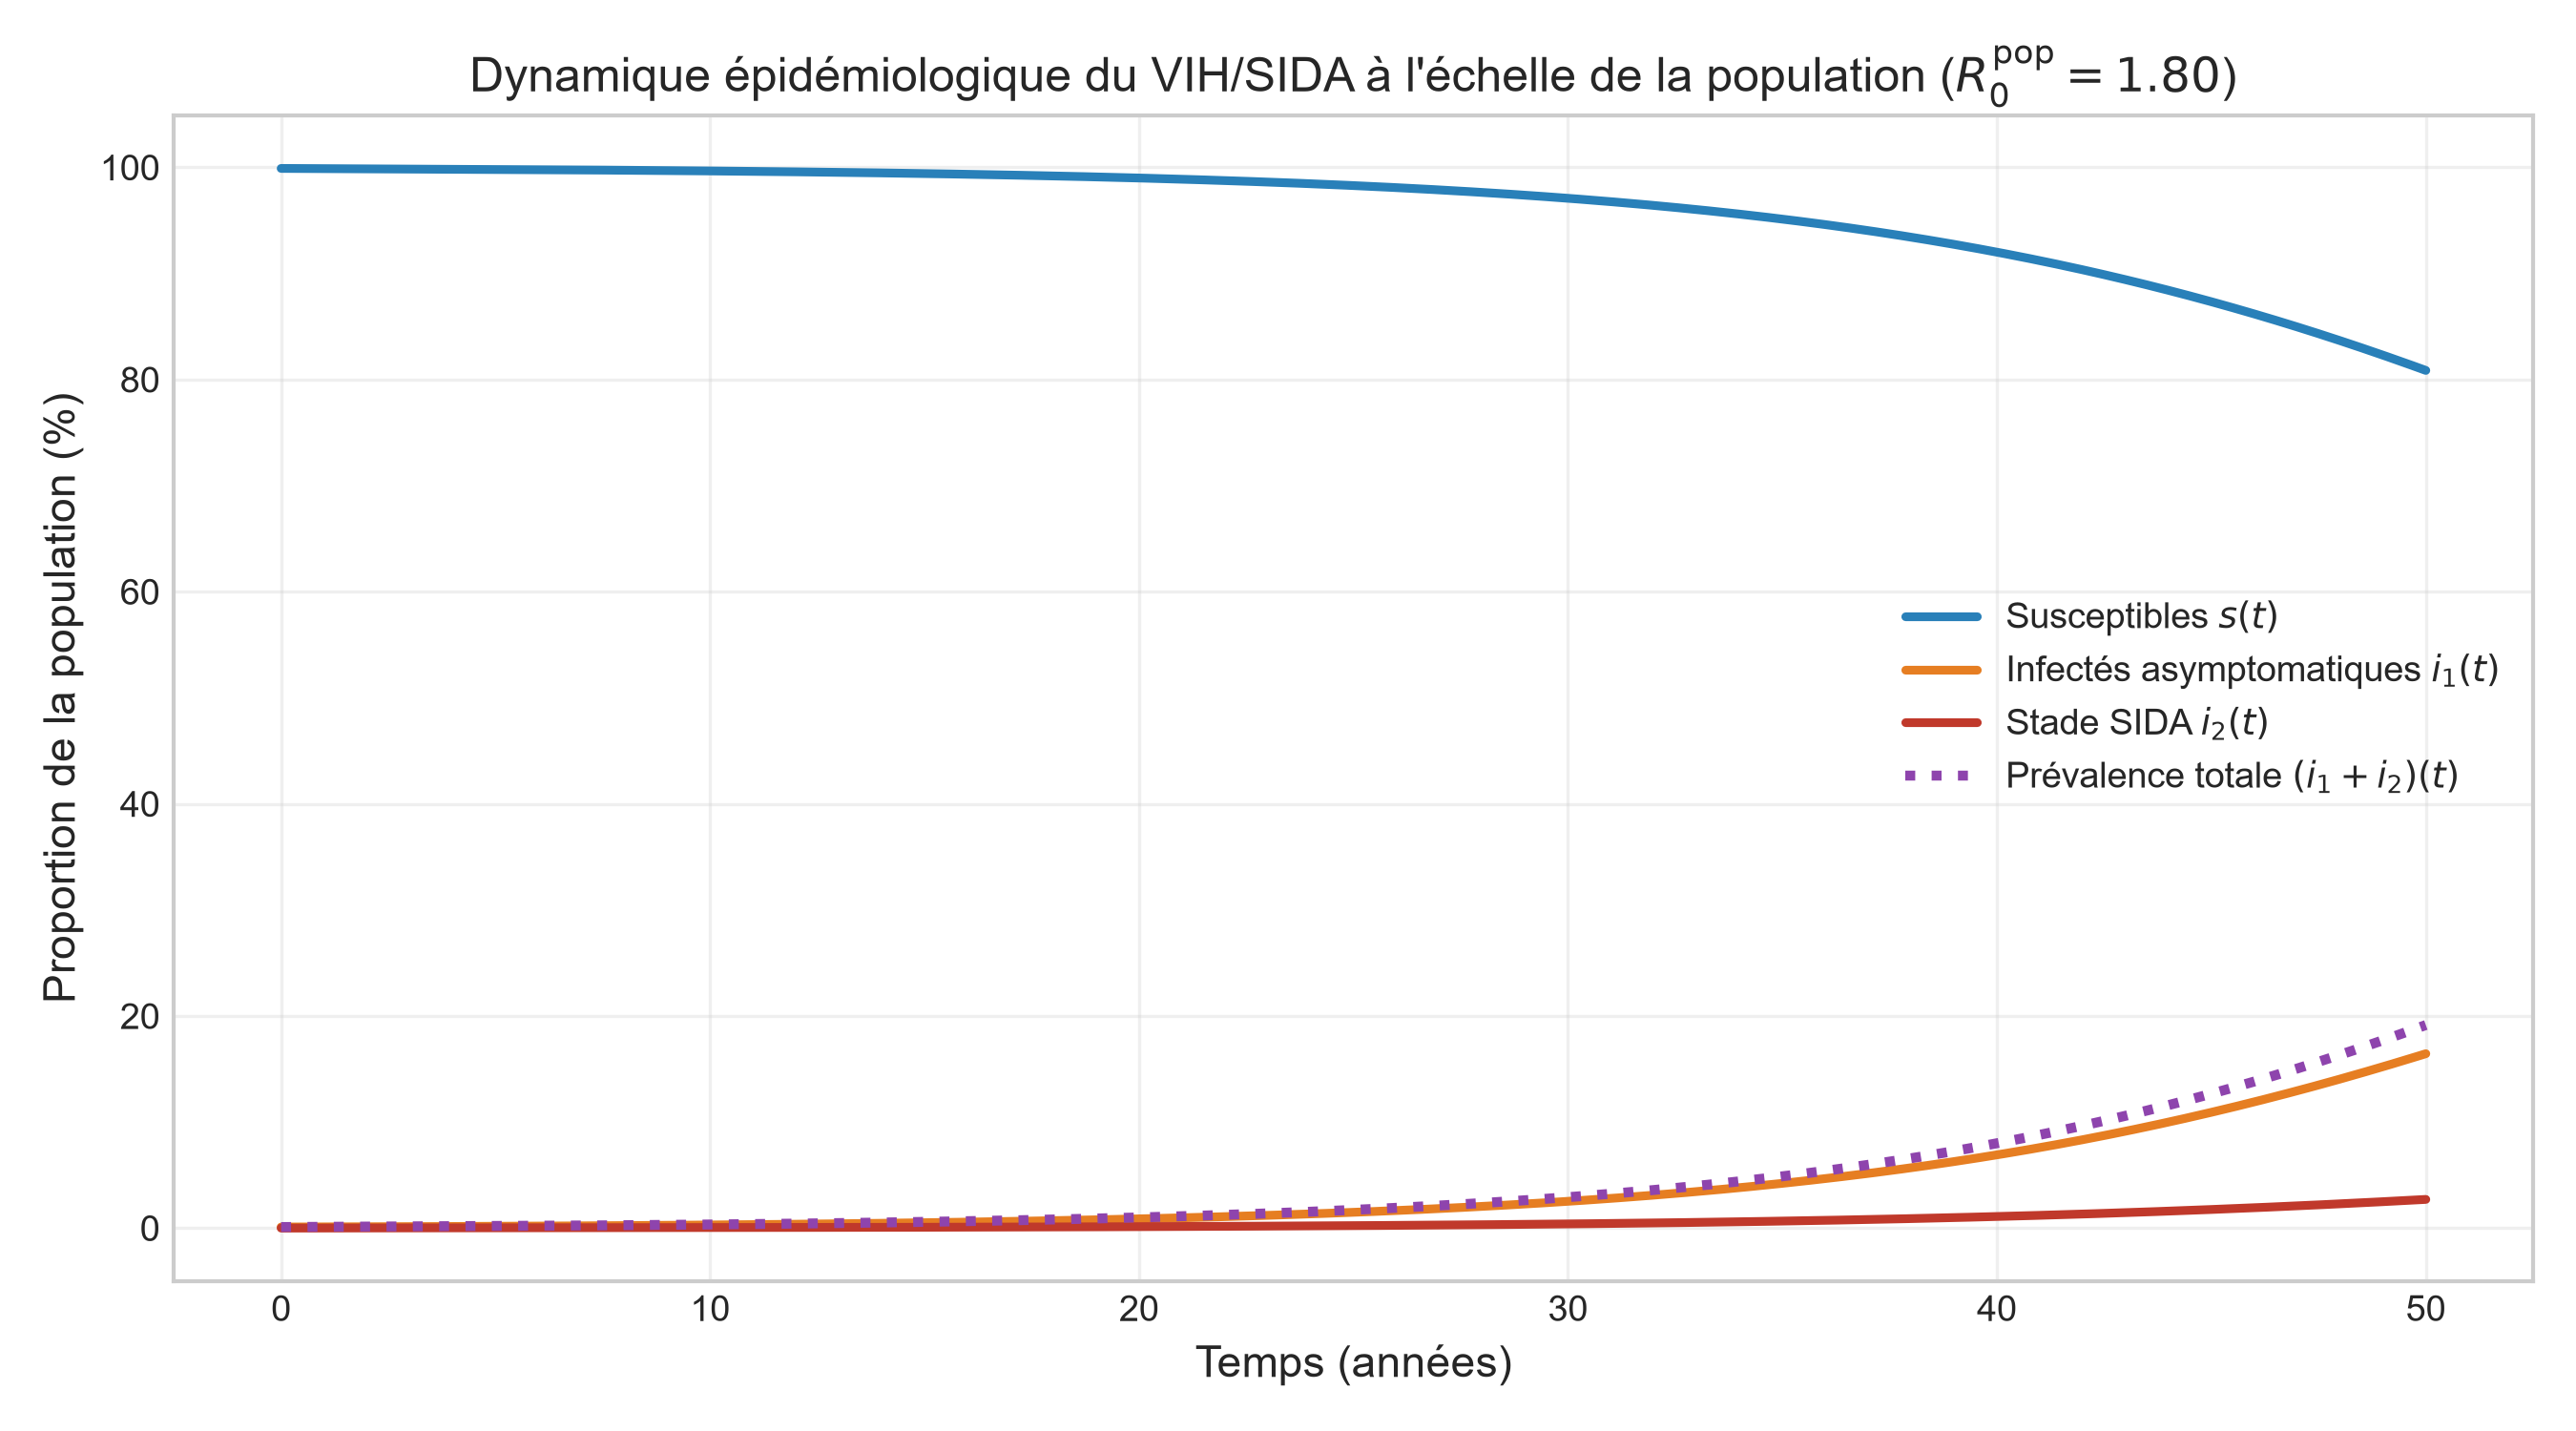
\includegraphics[width=\textwidth]{figures/fig16_population_dynamique.png}
    \caption{Dynamique épidémique sans intervention : proportions, prévalence et effectif total.}
    \label{fig:fig16_pop}
\end{minipage}
\hfill
\begin{minipage}{0.48\textwidth}
    \centering
    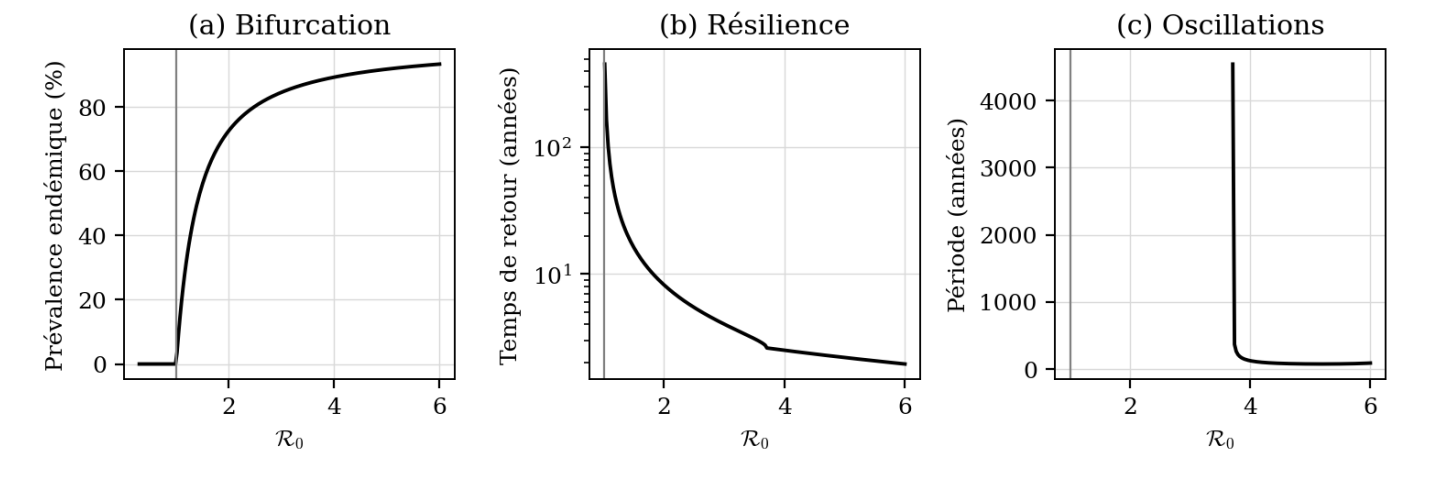
\includegraphics[width=\textwidth]{figures/fig17_bifurcation_pop.png}
    \caption{Bifurcation selon $\Rzero^{\mathrm{pop}}$ : prévalence endémique, temps de retour, période.}
    \label{fig:fig17_bif_pop}
\end{minipage}
\end{figure}

\noindent\textbf{Lecture des figures.} La figure~\ref{fig:fig16_pop} montre une croissance lente puis rapide de la prévalence vers son plateau d'environ $68\,\%$ (ordre de grandeur de plusieurs décennies pour atteindre l'essentiel du plateau). La figure~\ref{fig:fig17_bif_pop} confirme la bifurcation en $\Rzero^{\mathrm{pop}}=1$ (soit $\beta=\beta_c$) : en dessous, l'épidémie s'éteint ; au-dessus, la prévalence endémique croît avec $\Rzero$, et le temps de retour à l'équilibre diverge près du seuil (ralentissement critique).

\section{Scénarios d'intervention de santé publique}

On modélise trois interventions démarrant à l'an $30$ :
\begin{itemize}
    \item \textbf{Prévention} (préservatifs, éducation) : $\beta\to0{,}5\,\beta$ ;
    \item \textbf{Traitement} (antirétroviraux précoces) : la surmortalité liée au SIDA tombe de $\mu_2=0{,}5$ à $0{,}1$ ;
    \item \textbf{Combinaison} des deux.
\end{itemize}

\begin{table}[ht]
\centering
\caption{Scénarios d'intervention : $\Rzero^{\mathrm{pop}}$ et prévalence à long terme (simulation sur $300$ ans).}
\label{tab:scenarios}
\begin{tabular}{l c c}
\toprule
\textbf{Scénario} & $\Rzero^{\mathrm{pop}}$ & \textbf{Prévalence à $300$ ans} \\
\midrule
Sans intervention & $1{,}80$ & $67{,}8\,\%$ \\
Prévention seule ($\beta\times0{,}5$) & $0{,}90$ & $0{,}07\,\%$ \\
Traitement seul ($\mu_2=0{,}1$) & $2{,}07$ & $64{,}0\,\%$ \\
Prévention + traitement & $1{,}04$ & $4{,}6\,\%$ \\
\bottomrule
\end{tabular}
\end{table}

\begin{figure}[ht]
\centering
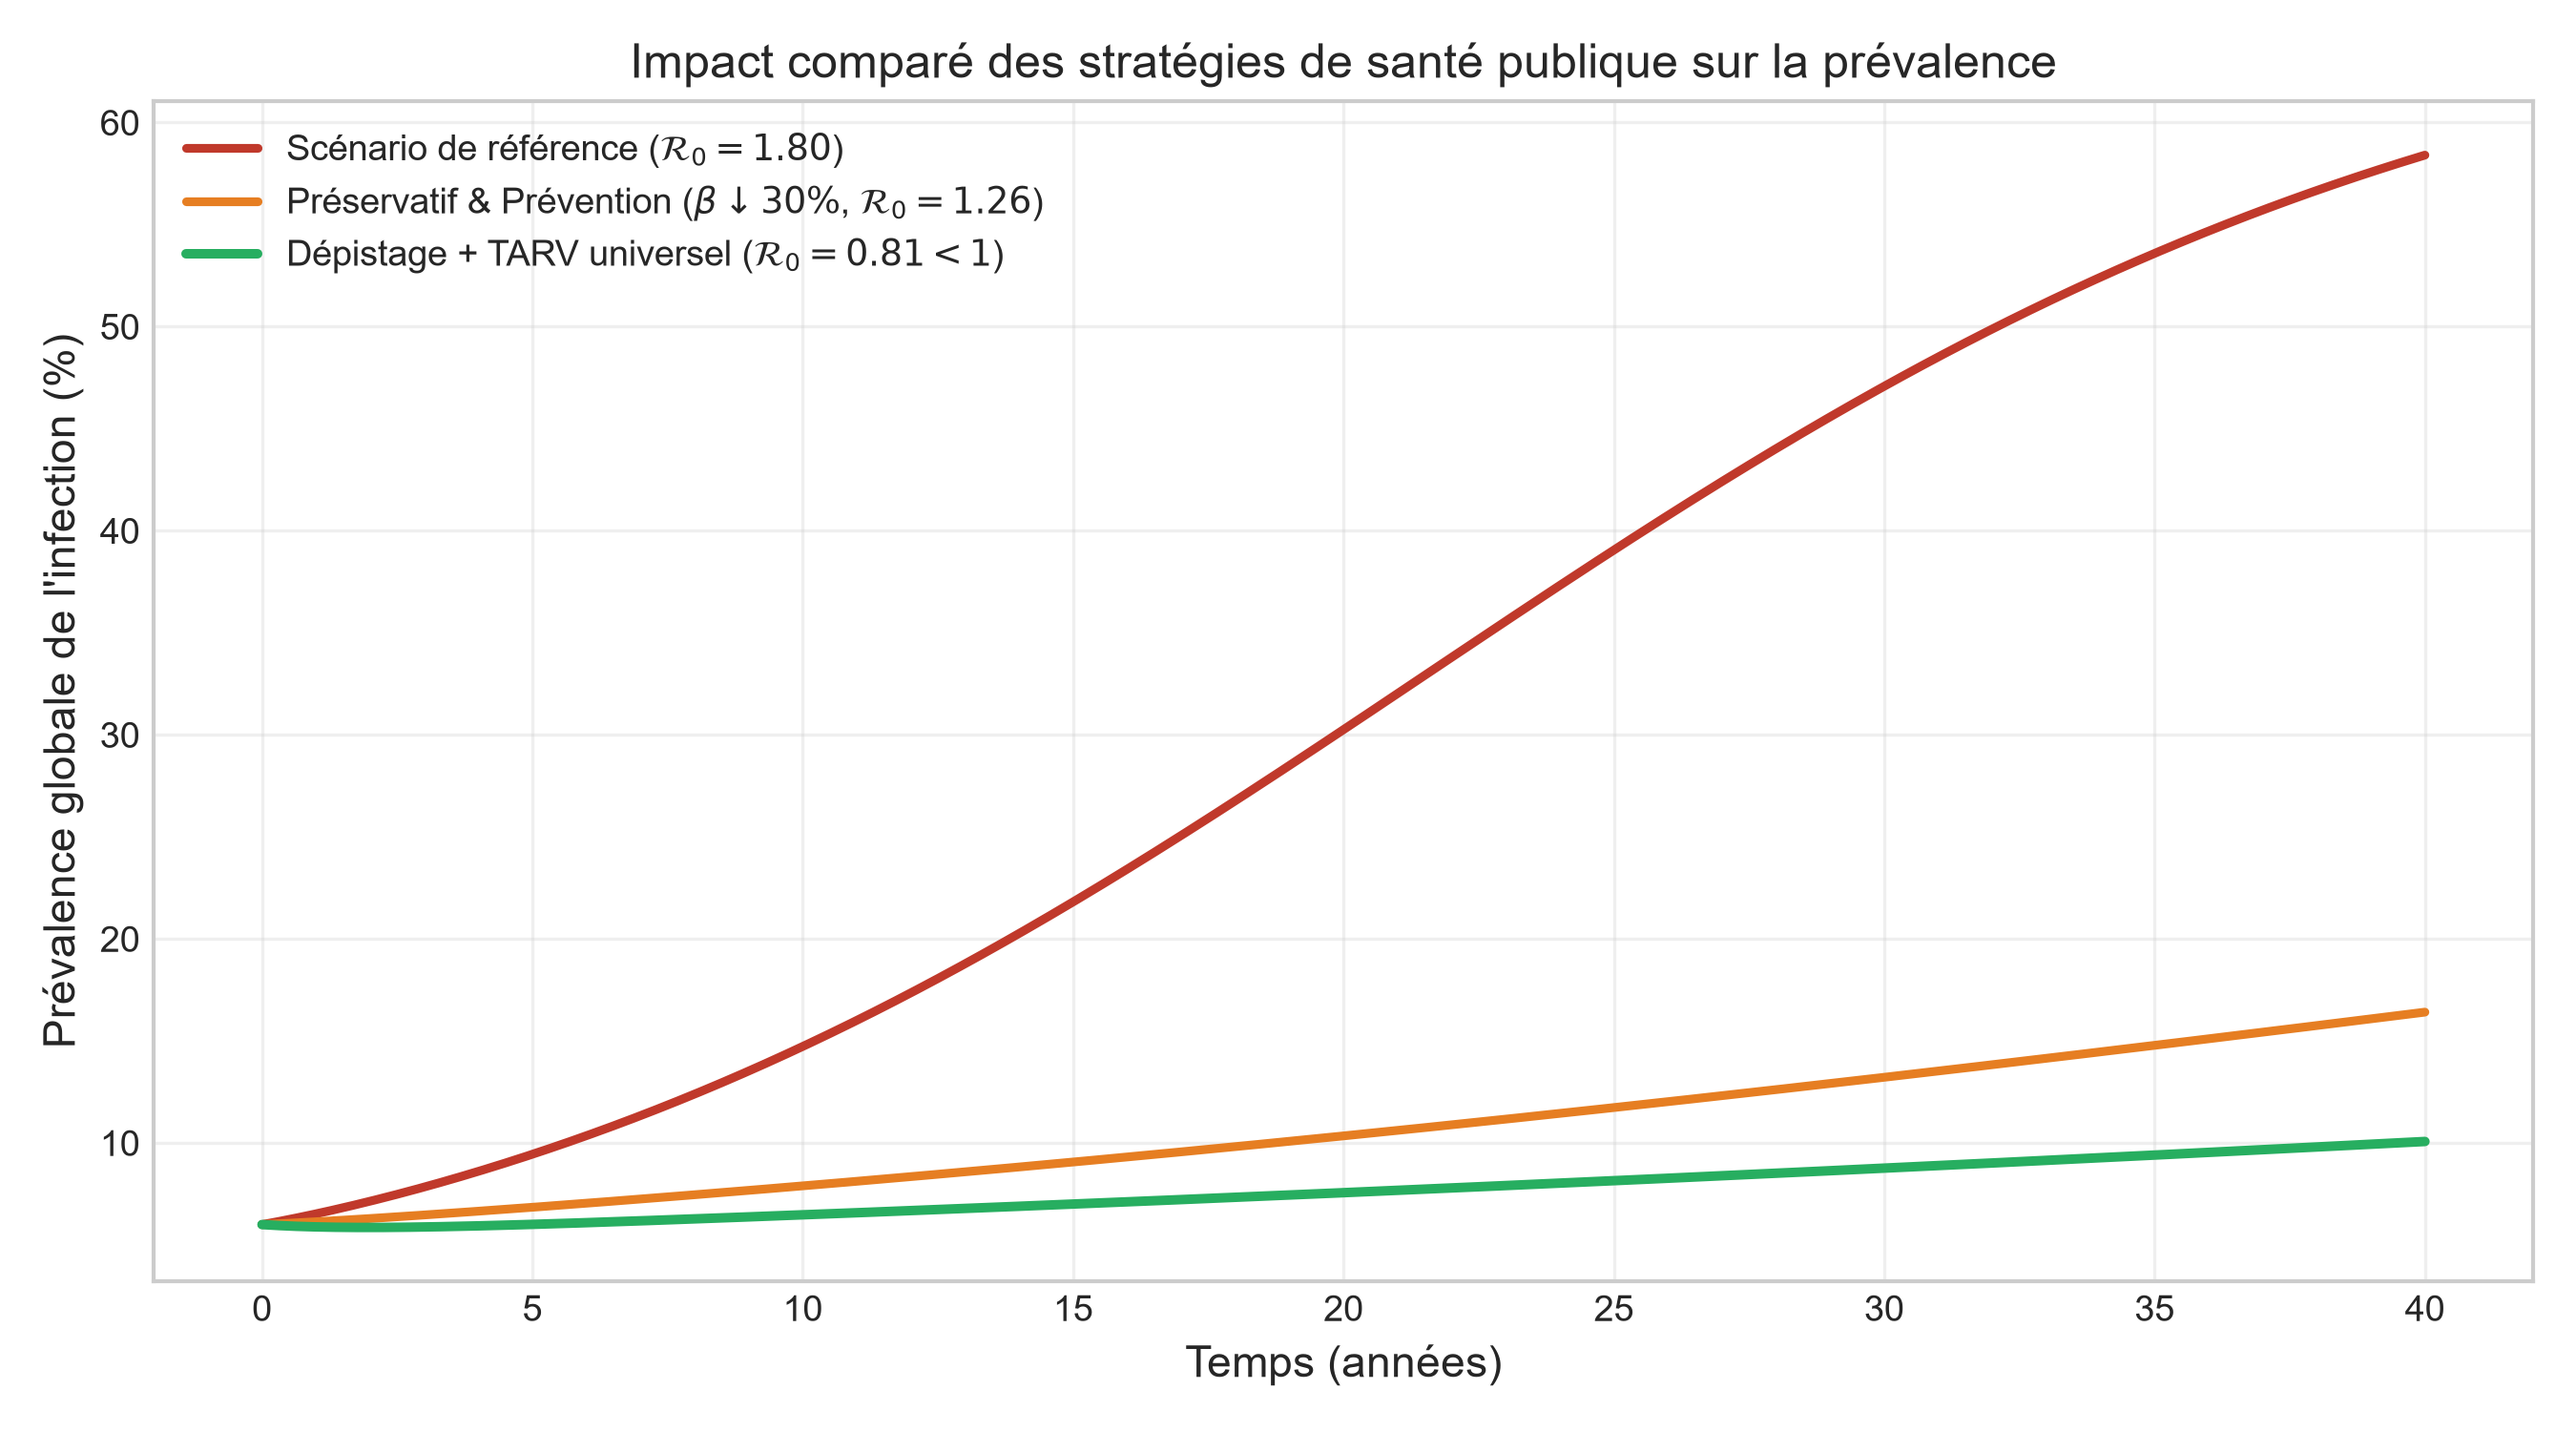
\includegraphics[width=0.85\textwidth]{figures/fig18_interventions.png}
\caption{Comparaison de scénarios de santé publique (prévalence et effectif total).}
\label{fig:fig18_scenarios}
\end{figure}

\noindent\textbf{Interprétation.} Les résultats du tableau~\ref{tab:scenarios} appellent trois remarques.
\begin{enumerate}
    \item Le traitement seul \emph{augmente} $\Rzero^{\mathrm{pop}}$ (de $1{,}80$ à $2{,}07$) dans ce modèle, car il prolonge la vie des individus infectés, donc leur période de contagiosité : il sauve des vies mais ne bloque pas la transmission et la prévalence reste élevée ($64\,\%$).
    \item La prévention seule, en divisant $\beta$ par deux, fait passer $\Rzero^{\mathrm{pop}}$ sous $1$ : l'épidémie s'éteint.
    \item La combinaison est ici \emph{moins} efficace que la prévention seule pour l'extinction, car le traitement allonge les durées d'infection ; avec $\Rzero^{\mathrm{pop}}=1{,}04$ juste au-dessus du seuil, la prévalence retombe à un niveau bas mais l'épidémie n'est pas éteinte et peut se maintenir longtemps.
\end{enumerate}
Il en ressort que, dans ce modèle, la prévention est le levier décisif, le traitement ayant surtout un bénéfice individuel (survie) et nécessitant d'être associé à des mesures de réduction de la transmission. Ce résultat dépend de l'hypothèse que le traitement n'affecte pas $\beta$ ; en réalité, un traitement efficace réduit aussi la contagiosité (voir les limites du modèle).

\begin{encadreresume}[Mini-résumé du chapitre 10 : modèle de population]
\begin{enumerate}
    \item Trois groupes : $S$, $I_1$ (asymptomatiques), $I_2$ (SIDA), avec incidence standardisée.
    \item $\Rzero^{\mathrm{pop}}=\frac{\beta}{\sigma+\Lambda_a}\big(1+\frac{\varepsilon\sigma}{\mu_2+\Lambda_a}\big)=1{,}8$ ; $\beta_c\approx0{,}133$ ; prévalence endémique $\approx68\,\%$.
    \item Prévention : décisive ($\Rzero=0{,}9$) ; traitement seul : prolonge la vie mais pas de contrôle de la transmission ($\Rzero=2{,}07$).
\end{enumerate}
\end{encadreresume}

% ==============================================================================
% CHAPITRE 11 : BENCHMARK
% ==============================================================================
\chapter{Benchmark haute performance BLAS / LAPACK}

\section{Protocole de mesure}

Le script \texttt{benchmark\_blas.py} (annexe~B) mesure :
\begin{itemize}
    \item le produit matriciel \texttt{DGEMM} (BLAS niveau~3), de coût $2n^3$ opérations flottantes ;
    \item la résolution de système \texttt{DGESV} (LAPACK), de coût $\frac23n^3$ ;
    \item des implémentations \textbf{Python naïf} (boucles et listes, fonctions \texttt{matmul\_naive} et \texttt{gauss\_naive}) servant de référence de comparaison.
\end{itemize}
Chaque mesure retient le \textbf{meilleur temps de plusieurs répétitions} (fonction \texttt{best\_time}) pour limiter l'effet du bruit système. Le débit est $\mathrm{GFLOPS}=\text{opérations}/(t\times10^9)$. Les matrices sont tirées avec un générateur aléatoire de graine fixée (\texttt{default\_rng(2026)}) et stockées en ordre Fortran. Le backend actif est identifié par \texttt{threadpoolctl} (section~4.1).

\begin{encadreattention}[Conditions de mesure du tableau et de la figure]
Les tableaux~\ref{tab:bench_speedup} et~\ref{tab:bench_gflops} ont été obtenus avec \texttt{benchmark\_blas.py} dans l'environnement suivant : processeur Intel Xeon à $2{,}8$ GHz (2 cœurs), Python~3.13, NumPy~2.5.3, SciPy~1.18.1, backend \textbf{OpenBLAS}~0.3.34. La figure~\ref{fig:fig19_bench} présente la même mesure effectuée sur la machine du groupe. Les valeurs absolues dépendent du matériel ; ce sont les ordres de grandeur et les tendances qui comptent.
\end{encadreattention}

\section{Résultats et analyse du gain de performance}

\paragraph{Gain par rapport à Python naïf.} Le tableau~\ref{tab:bench_speedup} compare, à même taille $n$, le code Python naïf et les routines BLAS/LAPACK.

\begin{table}[ht]
\centering
\caption{Temps d'exécution et facteur d'accélération (BLAS/LAPACK contre Python naïf).}
\label{tab:bench_speedup}
\begin{tabular}{c r r r r r r}
\toprule
 & \multicolumn{3}{c}{\textbf{Produit matriciel}} & \multicolumn{3}{c}{\textbf{Résolution $Ax=b$}} \\
\cmidrule(lr){2-4}\cmidrule(lr){5-7}
$n$ & Naïf (ms) & \texttt{DGEMM} (ms) & Gain & Naïf (ms) & \texttt{DGESV} (ms) & Gain \\
\midrule
$50$ & $6{,}3$ & $0{,}009$ & $\times 720$ & $2{,}6$ & $0{,}026$ & $\times100$ \\
$100$ & $45{,}8$ & $0{,}048$ & $\times 950$ & $19{,}6$ & $0{,}094$ & $\times210$ \\
$200$ & $380{,}8$ & $0{,}39$ & $\times 980$ & $142{,}5$ & $0{,}45$ & $\times310$ \\
\bottomrule
\end{tabular}
\end{table}

Le gain est de l'ordre de \textbf{$10^3$ pour le produit matriciel} et de \textbf{plusieurs centaines pour la résolution de système}, dès $n=200$. Il croît avec $n$ pour \texttt{DGESV} : le surcoût fixe de l'interpréteur Python (boucles, objets) pèse davantage lorsque le nombre d'opérations augmente, alors que les noyaux BLAS travaillent par blocs vectorisés. Le code naïf étant de complexité $O(n^3)$ avec une constante très élevée, il devient impraticable bien avant $n=1000$ (plusieurs minutes), ce qui n'est donc pas mesuré ici.

\paragraph{Passage à l'échelle.} Le tableau~\ref{tab:bench_gflops} donne les temps et débits de \texttt{DGEMM} et \texttt{DGESV} pour de grandes matrices (figure~\ref{fig:fig19_bench}).

\begin{table}[ht]
\centering
\caption{Temps et débit de \texttt{DGEMM} et \texttt{DGESV} pour de grandes tailles ($\text{OpenBLAS}$, 2 cœurs).}
\label{tab:bench_gflops}
\begin{tabular}{c r r r r}
\toprule
$n$ & \texttt{DGEMM} (ms) & GFLOPS & \texttt{DGESV} (ms) & GFLOPS \\
\midrule
$100$ & $0{,}04$ & $50{,}5$ & $0{,}09$ & $7{,}0$ \\
$200$ & $0{,}33$ & $49{,}2$ & $0{,}44$ & $12{,}1$ \\
$400$ & $2{,}57$ & $49{,}8$ & $2{,}76$ & $15{,}5$ \\
$800$ & $19{,}4$ & $52{,}8$ & $18{,}7$ & $18{,}3$ \\
$1600$ & $135{,}6$ & $60{,}4$ & $89{,}9$ & $30{,}4$ \\
\bottomrule
\end{tabular}
\end{table}

\begin{figure}[ht]
\centering
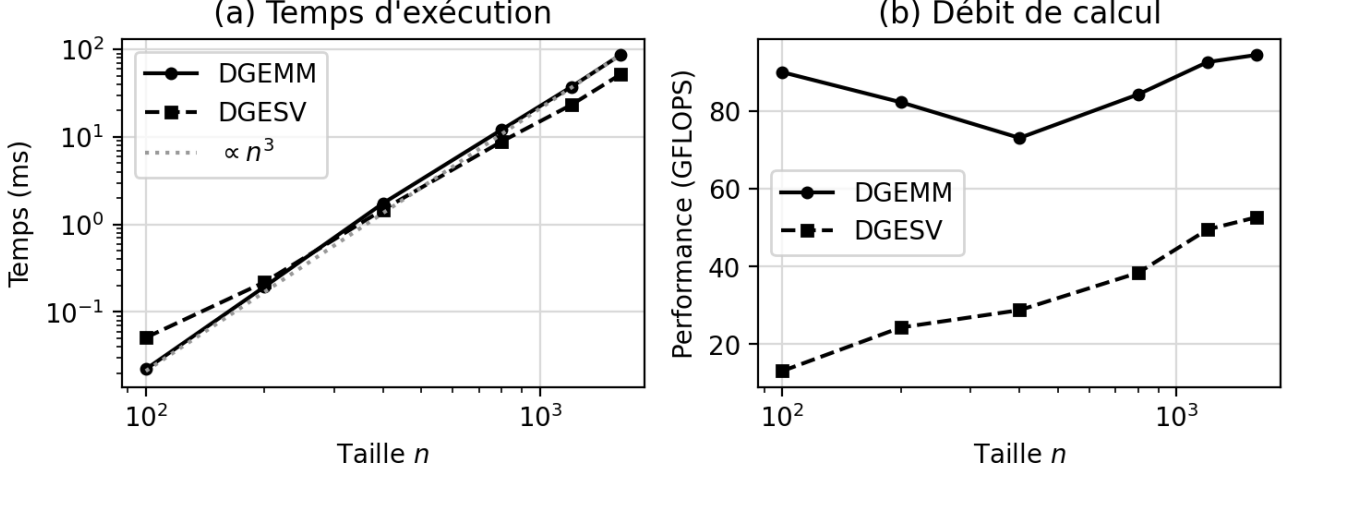
\includegraphics[width=0.85\textwidth]{figures/fig19_benchmark_perf.png}
\caption{Temps d'exécution (a) et débit en GFLOPS (b) de \texttt{DGEMM} et \texttt{DGESV} en fonction de $n$ (machine du groupe).}
\label{fig:fig19_bench}
\end{figure}

\paragraph{Analyse.}
\begin{itemize}
    \item \textbf{Loi en $n^3$.} Les temps croissent comme $n^3$ (droite de pente $3$ en échelle logarithmique), conformément aux coûts théoriques : multiplier $n$ par $2$ multiplie le temps par environ $8$.
    \item \textbf{\texttt{DGEMM} près de son régime stable.} Son débit varie peu avec $n$ : le niveau~3 est limité par le calcul, non par la mémoire (chapitre~2).
    \item \textbf{\texttt{DGESV} moins efficace que \texttt{DGEMM}, mais croissant.} Environ $\frac23n^3$ opérations dont une partie (la factorisation des panneaux) se fait au niveau~2, donc limitée par la mémoire ; la part de niveau~3 grandit avec $n$, d'où un débit croissant.
    \item \textbf{Rôle de la bibliothèque.} MKL et OpenBLAS appliquent les mêmes principes (blocage, vectorisation, multithreading) ; les écarts entre eux dépendent du processeur. L'exécution d'une comparaison directe OpenBLAS/MKL demande un environnement \texttt{conda} avec MKL ; elle n'a pas été réalisée ici.
\end{itemize}

\begin{encadreresume}[Mini-résumé du chapitre 11 : benchmark]
\begin{enumerate}
    \item BLAS/LAPACK sont environ $10^3$ fois plus rapides que le Python naïf pour le produit matriciel, et plusieurs centaines de fois pour la résolution de système, dès $n=200$.
    \item Les temps suivent la loi $n^3$ ; \texttt{DGEMM} atteint un débit presque constant, \texttt{DGESV} un débit croissant avec $n$.
    \item Les valeurs absolues dépendent du matériel et du backend (OpenBLAS ou MKL).
\end{enumerate}
\end{encadreresume}

% ==============================================================================
% CONCLUSION
% ==============================================================================
\chapter*{Conclusion et perspectives}
\addcontentsline{toc}{chapter}{Conclusion et perspectives}

Ce projet a mis en œuvre la chaîne complète qui mène d'un modèle biologique à une simulation numérique fiable :
\begin{enumerate}
    \item \textbf{Outils.} MKL, BLAS et LAPACK forment une pile cohérente : BLAS standardise les noyaux, LAPACK construit les solveurs par blocs, MKL ou OpenBLAS les optimise pour le matériel.
    \item \textbf{Modèle intra-hôte.} Il est borné et positif ; $\Rzero(\eta)=\frac{(1-\eta)\beta ps}{d\delta c}$ vaut $4$ sans traitement et fixe un seuil d'efficacité $\eta_c=75\,\%$. L'équilibre sain est globalement stable si $\Rzero\le1$ ; l'équilibre endémique est stable sinon, avec des oscillations de période $\approx53$ jours.
    \item \textbf{Numérique.} L'équilibrage \texttt{DGEEQU} ramène le conditionnement de la jacobienne de $10^5$ à quelques dizaines ; Newton + \texttt{DGESV} converge quadratiquement ; l'Euler implicite linéarisé surmonte la raideur et converge à l'ordre $1$.
    \item \textbf{Résultats médicaux.} Pic de virémie en primo-infection, élimination du virus pour $\eta>75\,\%$ et rebond d'environ $18$ fois le niveau chronique après arrêt du traitement.
    \item \textbf{Population.} $\Rzero^{\mathrm{pop}}=1{,}8$ ; la prévention est le levier décisif, le traitement seul ne bloquant pas la transmission dans ce modèle.
    \item \textbf{Performance.} Gain de l'ordre de $10^3$ pour \texttt{DGEMM} et de plusieurs centaines pour \texttt{DGESV} par rapport à Python naïf.
\end{enumerate}

\paragraph{Perspectives.} (i)~Utiliser un intégrateur raide d'ordre supérieur (BDF, Radau) ; (ii)~mesurer explicitement MKL contre OpenBLAS sur une même machine, avec variation du nombre de threads ; (iii)~étendre à des modèles spatiaux (équations aux dérivées partielles) en exploitant les solveurs LAPACK pour matrices bandes ; (iv)~comparer des exécutions sur GPU (cuBLAS).

\section*{Limites du modèle}

\begin{itemize}
    \item \textbf{Modèle intra-hôte :} il ignore la réponse immunitaire adaptative, les cellules latentes (réservoir), les mutations et résistances, et suppose une efficacité $\eta$ constante, une incidence bilinéaire et des paramètres identiques pour tous les patients. L'équilibre chronique ($V^*\approx650$ virions/$\mu$L) et les oscillations amorties qui l'entourent sont des propriétés de ce modèle simple, pas nécessairement des observations cliniques.
    \item \textbf{Modèle de population :} mélange homogène, pas de structure d'âge, de sexe ou de réseaux de partenaires ; un traitement n'y agit que sur la mortalité $\mu_2$, alors qu'il réduit aussi la contagiosité (ce qui modifierait la conclusion sur la combinaison) ; $\beta$ est \emph{calibré} pour imposer $\Rzero^{\mathrm{pop}}=1{,}8$, et non estimé sur des données réelles ; la natalité $\Lambda_a$ et la mortalité $\mu_a$ différentes impliquent un effectif total qui varie fortement sur de longues durées.
    \item \textbf{Numérique :} l'Euler implicite est d'ordre $1$ (précision limitée aux grands pas) ; les paramètres du tableau~\ref{tab:params_intra} sont des valeurs de littérature arrondies.
    \item \textbf{Benchmark :} résultats obtenus pour un matériel et un backend donnés ; la comparaison OpenBLAS/MKL reste à réaliser.
\end{itemize}

% ==============================================================================
% BIBLIOGRAPHIE
% ==============================================================================
\begin{thebibliography}{99}
\addcontentsline{toc}{chapter}{Références bibliographiques}
\bibitem{nowak2000} M. A. Nowak, R. M. May, \textit{Virus Dynamics: Mathematical Principles of Immunology and Virology}, Oxford University Press, 2000.
\bibitem{perelson1999} A. S. Perelson, P. W. Nelson, \textit{Mathematical analysis of HIV-1 dynamics in vivo}, SIAM Review 41(1), 1999, 3--44.
\bibitem{perelson1996} A. S. Perelson et al., \textit{HIV-1 dynamics in vivo: virion clearance rate, infected cell life-span, and viral generation time}, Science 271, 1996, 1582--1586.
\bibitem{diekmann1990} O. Diekmann, J. A. P. Heesterbeek, J. A. J. Metz, \textit{On the definition and the computation of the basic reproduction ratio $R_0$ in models for infectious diseases in heterogeneous populations}, J. Math. Biol. 28, 1990, 365--382.
\bibitem{vandendriessche2002} P. van den Driessche, J. Watmough, \textit{Reproduction numbers and sub-threshold endemic equilibria for compartmental models of disease transmission}, Math. Biosci. 180, 2002, 29--48.
\bibitem{korobeinikov2004} A. Korobeinikov, \textit{Global properties of basic virus dynamics models}, Bull. Math. Biol. 66, 2004, 879--883.
\bibitem{deleenheer2003} P. De Leenheer, H. L. Smith, \textit{Virus dynamics: a global analysis}, SIAM J. Appl. Math. 63(4), 2003, 1313--1327.
\bibitem{anderson1991} R. M. Anderson, R. M. May, \textit{Infectious Diseases of Humans: Dynamics and Control}, Oxford University Press, 1991.
\bibitem{lapack1999} E. Anderson et al., \textit{LAPACK Users' Guide}, 3e éd., SIAM, 1999.
\bibitem{blas1979} C. L. Lawson, R. J. Hanson, D. R. Kincaid, F. T. Krogh, \textit{Basic linear algebra subprograms for Fortran usage}, ACM TOMS 5(3), 1979, 308--323.
\bibitem{blas1990} J. J. Dongarra, J. Du Croz, S. Hammarling, I. S. Duff, \textit{A set of level 3 basic linear algebra subprograms}, ACM TOMS 16(1), 1990, 1--17.
\bibitem{goto2008} K. Goto, R. A. van de Geijn, \textit{Anatomy of high-performance matrix multiplication}, ACM TOMS 34(3), 2008, art.~12.
\bibitem{golub2013} G. H. Golub, C. F. Van Loan, \textit{Matrix Computations}, 4e éd., Johns Hopkins University Press, 2013.
\bibitem{higham2002} N. J. Higham, \textit{Accuracy and Stability of Numerical Algorithms}, 2e éd., SIAM, 2002.
\bibitem{hairer1996} E. Hairer, G. Wanner, \textit{Solving Ordinary Differential Equations II: Stiff and Differential-Algebraic Problems}, Springer, 1996.
\end{thebibliography}

% ==============================================================================
% ANNEXES
% ==============================================================================
\appendix

\chapter{Code source du mini-projet (\texttt{vih\_lapack.py})}

\section{Le module du modèle : \texttt{vih\_lapack.py}}

Ce module contient les outils LAPACK (\texttt{eigvals\_lapack}, \texttt{lu\_solve}, \texttt{cond1}, \dots), le modèle intra-hôte (\texttt{rhs\_h}, \texttt{jac\_h}, \texttt{ee\_h}, \texttt{newton\_h}) et le modèle de population (\texttt{f\_B}, \texttt{J\_B}).

\lstinputlisting[language=Python]{vih_lapack.py}

\section{Le script de simulation : \texttt{simulation\_intra.py}}

Ce script utilise le module précédent. Il implémente l'Euler implicite résolu par \texttt{DGESV}, l'Euler explicite, la solution de référence (solveur \texttt{Radau}) et reproduit les résultats numériques des chapitres~7, 8, 9 et~10 (conditionnement et équilibrage, ordre de convergence, primo-infection, traitement, rebond, scénarios de population).

\lstinputlisting[language=Python]{simulation_intra.py}

\chapter{Code source du benchmark (\texttt{benchmark\_blas.py})}

\lstinputlisting[language=Python]{benchmark_blas.py}

\chapter{Guide d'exécution et reproductibilité}

Ce guide permet à toute personne de refaire, pas à pas, les calculs du rapport. Les commandes sont données pour Linux/macOS (terminal) ; pour Windows, remplacer \texttt{python3} par \texttt{python} et utiliser l'invite de commandes ou PowerShell.

\section{Contenu du dossier}

\begin{lstlisting}[language={}]
Rapport_VIH_Groupe5/
|-- main.tex                 # source LaTeX du rapport
|-- figures/                 # figures (png) et logos
|-- vih_lapack.py            # modele + outils LAPACK (annexe A.1)
|-- simulation_intra.py      # simulations et verifications (annexe A.2)
|-- benchmark_blas.py        # benchmark BLAS/LAPACK (annexe B)
\end{lstlisting}

\section{Étape 1 : préparer l'environnement Python}

Il faut Python~3.9 ou plus récent. On crée un environnement isolé pour ne pas perturber le reste du système, puis on installe les bibliothèques :

\begin{lstlisting}[language={}]
cd Rapport_VIH_Groupe5
python3 -m venv env
source env/bin/activate            # Windows : env\Scripts\activate
pip install numpy scipy matplotlib threadpoolctl
\end{lstlisting}

\noindent Les quatre bibliothèques servent à : \texttt{numpy} (tableaux), \texttt{scipy} (accès à BLAS/LAPACK et solveur de référence), \texttt{matplotlib} (tracés, importé par le module), \texttt{threadpoolctl} (identification du backend et du nombre de threads).

\section{Étape 2 : vérifier la bibliothèque BLAS/LAPACK active}

\begin{lstlisting}[language={}]
python3 -c "from threadpoolctl import threadpool_info; \
[print(d['internal_api'], d['version'], d['num_threads']) \
 for d in threadpool_info()]"
\end{lstlisting}

\noindent Le programme affiche le nom du backend (\texttt{openblas} pour une installation par \texttt{pip}, \texttt{mkl} si l'environnement est configuré avec MKL), sa version et son nombre de threads. Notez ces informations : les temps du benchmark en dépendent.

\section{Étape 3 : tester le module du modèle}

\begin{lstlisting}[language={}]
python3 vih_lapack.py
\end{lstlisting}

\noindent Résultat attendu : \texttt{Modele VIH-SIDA avec LAPACK initialise avec succes.} Si une erreur d'importation apparaît, vérifier que l'environnement est activé et que l'étape~1 s'est bien terminée.

\section{Étape 4 : reproduire les résultats numériques}

\begin{lstlisting}[language={}]
python3 simulation_intra.py
\end{lstlisting}

\noindent Le script s'exécute en quelques secondes et affiche des blocs de résultats. Le tableau~\ref{tab:attendu} indique les valeurs que l'on doit retrouver (à l'arrondi près), avec la section du rapport correspondante.

\begin{table}[ht]
\centering
\caption{Résultats attendus de \texttt{simulation\_intra.py}.}
\label{tab:attendu}
\begin{tabularx}{\textwidth}{l X c}
\toprule
\textbf{Bloc affiché} & \textbf{Valeurs attendues} & \textbf{Section} \\
\midrule
$\Rzero$ et seuil & $\Rzero(0)=4{,}0$ ; $\eta_c=0{,}75$ & 6.2 \\
Équilibre endémique & $E^*=(250;\,15;\,652{,}17)$ & 6.3 \\
Valeurs propres en $E^*$ & $-23{,}50$ ; $-0{,}0197\pm0{,}1196\,i$ & 6.3 \\
Équilibrage \texttt{DGEEQU} & $\kappa_1(J(E^*))=1{,}5\times10^5\to\approx69$ & 7.2 \\
Ordre de convergence & ordre observé $\to1$ (de $4{,}1$ à $1{,}1$) ; erreur $0{,}18$ pour $h=0{,}0125$ & 8.2 \\
Stabilité à $h=0{,}1$ j & explicite : \texttt{nan} (divergence) ; implicite : fini & 8.2 \\
Point fixe à $t=600$ j & erreur relative $\approx10^{-5}$ & 8.2 \\
Primo-infection & pic $V\approx1{,}7\times10^4$ au jour $15{,}4$ ; $T_{\min}\approx49$ & 9.1 \\
Traitement & $\eta=0{,}95$ : indétectable au jour $\approx20$ ; $\eta=0{,}70$ : jour $\approx34$ puis remontée ($V\approx145$) & 9.2 \\
Arrêt du traitement & $T(100)\approx724$ ; rebond $\approx1{,}2\times10^4$, soit $18{,}5\times V^*$ & 9.2 \\
Scénarios (population) & $\Rzero=1{,}80\ /\ 0{,}90\ /\ 2{,}07\ /\ 1{,}04$ ; prévalence $67{,}8\ /\ 0{,}07\ /\ 64{,}0\ /\ 4{,}6\,\%$ & 10.3 \\
\bottomrule
\end{tabularx}
\end{table}

\noindent Des avertissements de dépassement de capacité (\texttt{RuntimeWarning: overflow}) apparaissent lors du test d'Euler explicite : c'est normal, ils illustrent la divergence décrite au chapitre~8.

\section{Étape 5 : refaire le benchmark}

\begin{lstlisting}[language={}]
python3 benchmark_blas.py
\end{lstlisting}

\noindent Le script affiche d'abord le backend détecté, puis, pour $n=100,200,400,800,1600$, le temps et le débit (GFLOPS) de \texttt{DGEMM} et \texttt{DGESV}, par exemple :

\begin{lstlisting}[language={}]
n=  100 | DGEMM:     0.04 ms ( 50.5 GFLOPS) | DGESV:     0.09 ms (  7.0 GFLOPS)
\end{lstlisting}

\noindent Les valeurs absolues dépendent de la machine : \textbf{ce sont les tendances qui doivent être reproduites} (temps en $n^3$, \texttt{DGEMM} plus rapide en GFLOPS que \texttt{DGESV}, débit croissant avec $n$). Pour fixer le nombre de threads :

\begin{lstlisting}[language={}]
OMP_NUM_THREADS=1 python3 benchmark_blas.py     # Linux / macOS
set OMP_NUM_THREADS=1 && python benchmark_blas.py   # Windows
\end{lstlisting}

\noindent Pour mesurer la scalabilité, répéter avec $1$, $2$, $4$ threads et comparer les temps de $n=1600$.

\section{Comparer avec Intel MKL}

Pour comparer OpenBLAS et MKL, créer un second environnement \texttt{conda} dont NumPy et SciPy sont liés à MKL, puis relancer l'étape~2 (le backend doit afficher \texttt{mkl}) et l'étape~5 :

\begin{lstlisting}[language={}]
conda create -n mkl python=3.11 numpy scipy matplotlib threadpoolctl "libblas=*=*mkl"
conda activate mkl
python3 benchmark_blas.py
\end{lstlisting}

\noindent Reporter ensuite les deux séries de temps dans un tableau côte à côte (même machine, même nombre de threads, plusieurs répétitions). Le nombre de threads de MKL se règle avec \texttt{MKL\_NUM\_THREADS}.

\section{Étape 6 : compiler le rapport}

\begin{lstlisting}[language={}]
pdflatex main.tex
pdflatex main.tex       # 2e passage : table des matieres et references
\end{lstlisting}

\noindent La compilation demande une distribution \LaTeX{} (TeX Live ou MiKTeX) avec le français pour \texttt{babel} (paquet \texttt{texlive-lang-french} sous Debian/Ubuntu ; MiKTeX l'installe automatiquement). Les figures du dossier \texttt{figures/} sont fournies déjà générées ; les chiffres que l'on peut recalculer sont ceux produits par \texttt{simulation\_intra.py} et \texttt{benchmark\_blas.py}.

\section{Problèmes fréquents}

\begin{table}[ht]
\centering
\caption{Dépannage.}
\begin{tabularx}{\textwidth}{p{5.2cm} X}
\toprule
\textbf{Symptôme} & \textbf{Cause probable et solution} \\
\midrule
\texttt{ModuleNotFoundError: vih\_lapack} & Lancer \texttt{simulation\_intra.py} depuis le dossier qui contient \texttt{vih\_lapack.py}. \\
\texttt{ModuleNotFoundError: scipy} (ou autre) & Environnement non activé, ou \texttt{pip install} non exécuté. \\
\texttt{AssertionError: DGESV a echoue} & Matrice singulière : vérifier les paramètres du modèle (dictionnaire \texttt{PA}). \\
Temps du benchmark très variables & Fermer les autres programmes ; augmenter le nombre de répétitions \texttt{rep} dans \texttt{best\_time}. \\
\texttt{Unknown option 'french'} à la compilation & Paquet de langue française de \TeX{} manquant : l'installer (voir étape~6). \\
\bottomrule
\end{tabularx}
\end{table}

\paragraph{Dépôt du projet.} \url{https://github.com/JuniorB573/OCS-Groupe5}

\end{document}
